\documentclass[reqno,12pt,letterpaper]{amsart}
\RequirePackage{amsmath,amssymb,amsthm,graphicx,mathrsfs,url,slashed}
\RequirePackage[usenames,dvipsnames]{color}
\RequirePackage[colorlinks=true,linkcolor=Red,citecolor=Green]{hyperref}
\RequirePackage{amsxtra}
\usepackage{cancel}
\usepackage{tikz-cd}

\setlength{\textheight}{9in} \setlength{\oddsidemargin}{-0.25in}
\setlength{\evensidemargin}{-0.25in} \setlength{\textwidth}{7in}
\setlength{\topmargin}{-0.25in} \setlength{\headheight}{0.18in}
\setlength{\marginparwidth}{1.0in}
\setlength{\abovedisplayskip}{0.2in}
\setlength{\belowdisplayskip}{0.2in}
\setlength{\parskip}{0.05in}
\renewcommand{\baselinestretch}{1.05}

\title[Least gradient maximum principle]{The maximum principle for functions of Riemannian least gradient}
\author{Aidan Backus}
\date{July 2021}

\newcommand{\NN}{\mathbf{N}}
\newcommand{\ZZ}{\mathbf{Z}}
\newcommand{\QQ}{\mathbf{Q}}
\newcommand{\RR}{\mathbf{R}}
\newcommand{\CC}{\mathbf{C}}
\newcommand{\DD}{\mathbf{D}}
\newcommand{\PP}{\mathbf P}
\newcommand{\MM}{\mathbf M}
\newcommand{\II}{\mathbf I}
\newcommand{\Hyp}{\mathbf H}
\newcommand{\Sph}{\mathbf S}

\DeclareMathOperator{\card}{card}
\DeclareMathOperator{\cent}{center}
\DeclareMathOperator{\ch}{ch}
\DeclareMathOperator{\codim}{codim}
\DeclareMathOperator{\diag}{diag}
\DeclareMathOperator{\diam}{diam}
\DeclareMathOperator{\dom}{dom}
\DeclareMathOperator{\Gal}{Gal}
\DeclareMathOperator{\Hom}{Hom}
\DeclareMathOperator{\Jac}{Jac}
\DeclareMathOperator{\Lip}{Lip}
\DeclareMathOperator{\Met}{Met}
\DeclareMathOperator{\id}{id}
\DeclareMathOperator{\rad}{rad}
\DeclareMathOperator{\rank}{rank}
\DeclareMathOperator{\Hess}{Hess}
\DeclareMathOperator{\Radon}{Radon}
\DeclareMathOperator*{\Res}{Res}
\DeclareMathOperator{\sgn}{sgn}
\DeclareMathOperator{\singsupp}{sing~supp}
\DeclareMathOperator{\Spec}{Spec}
\DeclareMathOperator{\supp}{supp}
\DeclareMathOperator{\Tan}{Tan}
\newcommand{\tr}{\operatorname{tr}}

\newcommand{\Ric}{\mathrm{Ric}}
\newcommand{\Riem}{\mathrm{Riem}}
\newcommand{\LapQL}{\Delta^{\mathrm{ql}}}

\newcommand{\dbar}{\overline \partial}

\DeclareMathOperator{\atanh}{atanh}
\DeclareMathOperator{\csch}{csch}
\DeclareMathOperator{\sech}{sech}

\DeclareMathOperator{\Div}{div}
\DeclareMathOperator{\Gram}{Gram}
\DeclareMathOperator{\grad}{grad}
\DeclareMathOperator{\Ell}{Ell}
\DeclareMathOperator{\WF}{WF}

\newcommand{\Lagrange}{\mathscr L}
\newcommand{\DirQL}{\mathscr D^{\mathrm{ql}}}
\newcommand{\DirL}{\mathscr D}

\newcommand{\Hilb}{\mathcal H}
\newcommand{\Homology}{\mathrm H}
\newcommand{\normal}{\mathbf n}
\newcommand{\vol}{\mathrm{vol}}

\newcommand{\pic}{\vspace{30mm}}
\newcommand{\dfn}[1]{\emph{#1}\index{#1}}

\renewcommand{\Re}{\operatorname{Re}}
\renewcommand{\Im}{\operatorname{Im}}

\def\Japan#1{\left \langle #1 \right \rangle}

\newtheorem{theorem}{Theorem}[section]
\newtheorem{badtheorem}[theorem]{``Theorem"}
\newtheorem{prop}[theorem]{Proposition}
\newtheorem{lemma}[theorem]{Lemma}
\newtheorem{claim}[theorem]{Claim}
\newtheorem{proposition}[theorem]{Proposition}
\newtheorem{corollary}[theorem]{Corollary}
\newtheorem{conjecture}[theorem]{Conjecture}
\newtheorem{axiom}[theorem]{Axiom}
\newtheorem{assumption}[theorem]{Assumption}

\theoremstyle{definition}
\newtheorem{definition}[theorem]{Definition}
\newtheorem{remark}[theorem]{Remark}
\newtheorem{example}[theorem]{Example}
\newtheorem{notation}[theorem]{Notation}

\newtheorem{exercise}[theorem]{Discussion topic}
\newtheorem{homework}[theorem]{Homework}
\newtheorem{problem}[theorem]{Problem}

\newtheorem{ack}{Acknowledgements}

\numberwithin{equation}{section}


% Mean
\def\Xint#1{\mathchoice
{\XXint\displaystyle\textstyle{#1}}%
{\XXint\textstyle\scriptstyle{#1}}%
{\XXint\scriptstyle\scriptscriptstyle{#1}}%
{\XXint\scriptscriptstyle\scriptscriptstyle{#1}}%
\!\int}
\def\XXint#1#2#3{{\setbox0=\hbox{$#1{#2#3}{\int}$ }
\vcenter{\hbox{$#2#3$ }}\kern-.6\wd0}}
\def\ddashint{\Xint=}
\def\dashint{\Xint-}

%\usepackage{color}
%\hypersetup{%
%    colorlinks=true, % make the links colored%
%    linkcolor=blue, % color TOC links in blue
%    urlcolor=red, % color URLs in red
%    linktoc=all % 'all' will create links for everything in the TOC
%Ning added hyperlinks to the table of contents 6/17/19
%}

% style=alphabetic
\usepackage[backend=bibtex,maxcitenames=50,maxnames=50]{biblatex}
\addbibresource{topics.bib}
\renewbibmacro{in:}{}
\DeclareFieldFormat{pages}{#1}

\begin{document}
\begin{abstract}
Topics exam, Fall 2021.
\end{abstract}

\maketitle

%%%%%%%%%%%%%%%%%%%%%%%%%%%%%%%%%%%%%%%%%%%%%%%%%%%%%%%

% \tableofcontents

\section{Introduction}
Let $M$ be an oriented Riemannian manifold of metric $g$ and dimension $d$.

\begin{definition}\label{main definitions}
A function $u$ of locally bounded variation has \dfn{least gradient} if for every compactly supported function $v$ of bounded variation, such that $\supp v \subseteq U \Subset M$,
$$\int_U |du| ~\vol \leq \int_U |du + dv| ~\vol.$$
A set $U$ of locally finite perimeter has \dfn{least perimeter} if $1_U$ has least gradient.
\end{definition}

\begin{definition}
A \dfn{minimal lamination} in $M$ is a partition of a closed subset of $M$ into smooth hypersurfaces with zero mean curvature.
The minimal lamination $\lambda$ is \dfn{analytic} if $(M, g)$ is analytic and each of the hypersurfaces in $\lambda$ is analytic.
\end{definition}

This paper is dedicated to the proof of the following generalization of the maximum principle for least gradient functions on euclidean space \cite[Proposition 3.4]{górny2017planar}.

\begin{theorem}[maximum principle]\label{main thm}
Suppose that $2 \leq d \leq 7$ and
\begin{enumerate}
\item either $g$ has constant sectional curvature $\leq 0$,
\item or $g$ has constant curvature and $d = 2$.
\end{enumerate}
Let $u: M \to \RR$ be a function of least gradient, and $A_y = \partial \{u > y\}$.
Then $(A_y)_{y \in \RR}$ is a minimal lamination, which is analytic if $(M, g)$ is.
\end{theorem}

We are primarily concerned with the case that $M$ is a closed hyperbolic manifold, which is the setting of several erstwhile open problems stated in \cite[\S9]{daskalopoulos2020transverse} which Theorem \ref{main thm} can be used to solve. See \S\ref{duality}.

If $d = 2$, then Theorem \ref{main thm} can be extended to manifolds with boundary, just as in \cite[Corollary 3.5]{górny2017planar}:

\begin{theorem}[maximum principle up to the boundary]\label{main crly}
Let $\overline \Sigma$ be a convex surface with boundary and suppose that $u: \Sigma \to \RR$ is a function of least gradient defined on the interior $\Sigma$ of $\overline \Sigma$.
Then, if $A_y = \partial \{u > y\}$, $(A_y)_{y \in \RR}$ extends to a geodesic lamination of $\overline \Sigma$.
\end{theorem}

Theorems \ref{main thm} and \ref{main crly} can be easily shown to follow from standard results and the following regularity theorem for sets of least perimeter, which is the main theorem of the present paper:

\begin{theorem}[regularity of minimal hypersurfaces]\label{main lma}
Suppose that $2 \leq d \leq 7$ and
\begin{enumerate}
\item either $g$ has constant sectional curvature $\leq 0$,
\item or $g$ has constant curvature and $d = 2$.
\end{enumerate}
Then every set of least perimeter is bounded by a smooth minimal hypersurface $N$.
Furthermore, $N$ is analytic if $(M, g)$ is.
\end{theorem}

A proof of an analogous result to Theorem \ref{main lma} for currents paired against an elliptic integrand is given by \cite[\S5.3]{federer2014geometric}; our proof uses a similar strategy but is rather ``hands-on" in that it avoids the use of homological integration, instead using the theory of functions of bounded variation as developed by Miranda in \cite{Miranda64} \cite{Miranda66} \cite{Miranda67}, and facts about minimal hypersurfaces in euclidean space.

Though the hypotheses of Theorem \ref{main lma} look odd, we only use the assumption of nonpositive curvature at a critical point to deduce that a certain elliptic operator which we construct is actually the euclidean Laplace operator when written in correctly chosen coordinates.
In general, such an operator would be a perturbation of the euclidean Laplacian and so a suitable analysis of perturbations of elliptic operators should extend all of our results to the case of constant sectional curvature, so it is reasonable to conjecture the following:

\begin{conjecture}\label{main conj}
Suppose that $2 \leq d \leq 7$ and $g$ has constant sectional curvature.
Then the level sets of a function of least gradient are a minimal lamination.
\end{conjecture}

The assumption of constant sectional curvature should be somewhat harder to remove, as we rely on the existence of certain Killing fields, and at one point use the Killing-Hopf theorem to reduce a general result to the euclidean case.
However, if one could show Conjecture \ref{main conj}, a proof for any Riemannian manifold of appropriate dimension should not be out of reach.

%%%%%%%%%%%%%%%%%%%%%%%%%%%%%%%%%%%%%%%%%%%%%%%

\subsection{Outline of the paper}
We begin with the preliminaries.
In \S\ref{RiemMeasureThy}, we record facts that we will use about sets of locally finite perimeter on Riemannian manifolds.
We introduce the notion of a \dfn{bundle-valued Radon measure}, which is a generalized section of a vector bundle that, upon trivialization, becomes a vector-valued Radon measure.
With the basic theory of bundle-valued Radon measures it is easy to show that the reduced boundary of a set of least perimeter is independent of the choice of metric.
We also show that a coarea formula holds in this setting, which we use in \S\ref{LeastGradientFunctions} to develop the theory of functions of least gradient on Riemannian manifolds. A generalization of Miranda's theorem \cite[Teorema 3]{Miranda67} on the stability of functions of least gradient, and generalizations of its standard consequences, easily fall out from the coarea formula.
We then focus on sets of least perimeter: we prove a monotonicity formula, compute the dimension of the reduced boundary as $d - 1$, and prove the existence of tangent spaces to the reduced boundary.

We are then ready to prove Theorem \ref{main lma}.
In \S\ref{MollifierSection}, we show Proposition \ref{mollifier proposition}, which says that a set of least perimeter can be approximated by $C^1$ hypersurfaces that are approximately minimal.
This result is then used in \S\ref{DeGiorgiSection}, to prove a generalization, Proposition \ref{de Giorgi}, of the de Giorgi regularity lemma \cite[Teorema 5.7]{Miranda66} for sets of least perimeter.
Most of the difficulty in this step, and indeed in this present paper, comes from proving the $C^1$ case of de Giorgi's lemma, as Proposition \ref{mollifier proposition} can be used to reduce Proposition \ref{de Giorgi} to this case.

In the euclidean case, the $C^1$ de Giorgi lemma is proven by comparing the surface area of the graph of a $C^1$ function $\omega$ to its Dirichlet energy $\int |d\omega|^2~\vol$, and then apply the mean-value property and the fact that $[\Delta, \partial_j] = 0$.
This does not quite work in general, as the commutator of the Laplace-Beltrami operator with a coordinate vector field will in general be nonzero, and the mean-value theorem only approximately holds for general Laplace-Beltrami operators.
Our main innovation here is to show that for a suitable space form, one has enough Killing fields to carry out a similar argument, in which the Dirichlet energy is actually the Lagrangian for the euclidean Laplacian.

In \S\ref{proof of main thm}, we use a standard inductive argument to show that Proposition \ref{de Giorgi} implies Theorem \ref{main lma}.
We then use Theorem \ref{main lma} and the general theory developed in \S\ref{LeastGradientFunctions} to prove Theorems \ref{main thm} and \ref{main crly}.

In \S\ref{duality}, we use Theorem \ref{main thm} to use certain conjectures of Daskalopoulos and Uhlenbeck \cite{daskalopoulos2020transverse}.

%%%%%%%%%%%%%%%%%%%%%%%%%%%%%%%%%%%%%%%%%%%%%%%%

\subsection{Acknowledgements}
I would like to thank Georgios Daskalopoulos for suggesting this project and for many helpful discussions.
I would also like to thank Joshua Lin for helpful discussions and in particular for suggesting the proof of Lemma \ref{cross product formula}.

%%%%%%%%%%%%%%%%%%%%%%%%%%%%%%%%%%%%%%%%%%%%%%%%%%%%%%%%%%%%%%%%%%%%%%%%%%%%%%%%%%%%%%%%%

\section{Riemannian measure theory}\label{RiemMeasureThy}
\subsection{Notation and conventions}
\begin{notation}[presheaves]
If $F$ is a presheaf of function spaces, we write $u \in F_l(U)$ to mean that for every $V \Subset U$, $u \in F(V)$.
We write $u \in F_c(U)$ to mean that $u \in F(U)$ and $\supp u \Subset U$.
\end{notation}

\begin{notation}[volume forms]
We reserve the letter $d$ for dimension or exterior differentiation, and so to avoid awkwardness such as $\int |du| dV$ we write $\vol$ for the Riemannian volume form.
If $N$ is a closed submanifold we write $\vol_N$ to indicate the pullback of $\vol$ along the inclusion map $M \to N$.
\end{notation}

\begin{notation}[vector bundles]
Let $E$ be a vector bundle, which we will always assume is normed, with dual $E'$.
If $u,v$ are sections of $E',E$ respectively, we write $(u, v)$ for their fiberwise pairing, which is a function $M \to \RR$.
We write $\langle u, v\rangle$ or $\int_M (u, v) ~\vol$, for their $L^2$-duality pairing, which is a real number.
If $u$ is a section of $E$, we write $u \prec U$ to mean that $||u||_{L^\infty} \lesssim 1$ and $\supp u \Subset U$.
\end{notation}

\begin{notation}[Einstein summation]\label{EinsteinNotation}
We will have occasion to use the Einstein summation convention on a manifold which, in the smooth category, can be expressed as a product $H \times I$ where $H$ is $d-1$-dimensional and $I$ is $1$-dimensional.
Latin indices range over $1, \dots, d - 1$ and index coordinate directions on $H$; Greek indices range over $0, \dots, d - 1$, and the $0$th coordinate is the coordinate on $I$.
However, we stress that the metric on $H \times I$ is Riemannian rather than Lorentzian.
\end{notation}

\begin{definition}
Let $u$ be a smooth section.
Then $u$ is \dfn{as smooth as possible} if either $u$ is analytic or $g$ is not analytic.
\end{definition}

%%%%%%%%%%%%%%%%%%%%%%%%%%%%%%%%%%%%%%%%%%%%%%%%%%%%%%%%%%%%

\subsection{The Bochner integral}
Let $F$ be a separable Fr\'echet space over $\CC$, and $(\Omega, P)$ a measure space.
We can then define the \dfn{Bochner integral} of a $P$-measurable function $f: \Omega \to F$, which we write as $\int_\Omega f ~dP \in F$.
See \cite{Rieffel70}, \cite{MO47721}, and \cite[Chapter V]{yosida2012functional}.
We recall a few facts that we will need:

\begin{theorem}[Pettis]
Let $f: \Omega \to F$ be any function.
Then $f$ is $P$-measurable iff for every $X \in F'$, $\omega \mapsto \langle f(\omega), X\rangle$ is $P$-measurable.
In this case,
$$\left\langle \int_\Omega f ~dP, X\right\rangle = \int_\Omega \langle f(\omega), X\rangle ~dP(\omega).$$
If $F = \CC^r$, then the Bochner integral is just the componentwise Lebesgue integral.
\end{theorem}

%%%%%%%%%%%%%%%%%%%%%%%%%%%%%%%%%%%%%%%%%%%%%%%%%%%%%%%%%%%%

\subsection{Bundle-valued Radon measures}
Let $F \to M$ be a normed vector bundle of rank $r$.
We equip the space $C(K, F)$ of continuous sections of $F$ on a compact set $K$ with its supremum norm.
The Banach spaces $C(K, F)$ form an inverse system with respect to restriction and therefore define the topological vector space
$$C_0(M, F) = \varprojlim C(K, F).$$

According to the Riesz-Markov theorem, the space of $\CC^r$-valued Radon measures on $M$ is canonically identified with $C_0(M, (\CC^r)')'$, thus we define:

\begin{definition}
The topological dual space $\mathcal R(M, F) = C_0(M, F')'$ is the space of \dfn{$F$-valued Radon measures} on $M$.
\end{definition}

If we write $\mathcal R(U, F)$ to mean $\mathcal R(U, F|U)$, we equip $\mathcal R(U, F)$ with the weak topology of measures.
Then $\mathcal R(U, F)$ is a separable Fr\'echet space, with seminorms $|\langle \cdot, f_j\rangle|$ where $(f_j)$ is a countable basis for a dense subspace of $C_0(U, F)$.
Thus $\mathcal R(\cdot, F)$ is a sheaf of separable Fr\'echet spaces.

\begin{definition}
If $\omega \in \mathcal R(M, F)$ we define the \dfn{total variation} $|\omega|$ to be the positive Radon measure such that on every open set $U$,
$$|\omega|(U) = \sup_{X \prec U} \langle \omega, X\rangle,$$
where $X$ ranges over $C_0(M, F')$.
\end{definition}

Since $\RR_+$ acts on $F$ by scalar multiplication, we can define the \dfn{sphere bundle} $SF = (F \setminus 0)/\RR_+$.
Since $F$ has a norm, $SF$ is naturally identified with the bundle of elements of $F$ with length $1$.

\begin{proposition}[Riesz-Markov representation]\label{HanhJordan}
Let $\omega$ be a $F$-valued Radon measure and let $\mu = |\omega|$.
Then there exists a $\mu$-measurable section $f$ of $SF$ such that for every section $X \in C_0(M, F', \mu)$,
\begin{equation}\label{RNy formula}
\langle \omega, X\rangle = \int_M (f, X) ~d\mu.
\end{equation}
Furthermore, $f$ is unique up to a $\mu$-null set, and does not depend on the norm of $F$.
\end{proposition}
\begin{proof}
Fix an open cover $(U_i)$ of $M$ by charts which trivialize $F$, so that $U_i$ is precompact in $M$.
Let $(g_{ij})$ be the transition functions and $(g_{ij}')$ the induced transition functions for the dual bundle $F'$.
Then can view $\omega_i = \omega|U_i$ as an element of $C(U_i, (\CC^r)')'$, by the precompactness of $U_i$.
Hence by the Riesz-Markov theorem \cite[Theorem 4.14]{simon1983GMT}, there exists a $\mu$-measurable section $f_i$ of $SF$ for which (\ref{RNy formula}) holds for $\omega_i$, provided that $X \in C(U_i, (\CC^r)')$.

We now show that the $f_i$ are restrictions of a global section $f$, thus we must show $f_j = g_{ij} \circ f_i$ on $\CC^r$.
To this end, fix $X \in C_0(M, F)$ which is supported in $U_i \cap U_j$ and write $X_i \in C(U_i, (\CC^r)')$ for the trivialization of $X$ with respect to $U_i$.
Then $X_j = g_{ij}' \circ X_i$, and
\begin{align*}
\int_E (f_i, X_i) ~d\mu &= \langle \omega_i, X_i\rangle = \langle \omega_j, X_j\rangle = \int_E (f_j, X_j) ~d\mu = \int_E (f_j, g_{ij}' \circ X_i) ~d\mu.
\end{align*}

By Urysohn's lemma, $C_c(U_i \cap U_j, (\CC^r)', \mu)$ separates points in $L^1(U_i \cap U_j, \CC^r, \mu)$.
Therefore, since $X$ was arbitrary, $f_i = g_{ji} \circ f_j$; thus we obtain a unique global section $f$ of $SF$.

Finally, if we change the norm of $F$, replacing $|\cdot|$ with $|\cdot|'$, then we obtain a smooth function $h: F \to \RR_+$ so that if $v \in F_x$, then $|v|' = h(x, v)|v|$.
The change of norm gives us a new section $f'$ such that $f' = f/h(\cdot, f'(\cdot))$.
Thus $f'$ defines the same section of $SF$ as $f$.
\end{proof}

At this stage we have only defined $f$ as a $\mu$-equivalence class of sections of $SF$, so we now use the Lebesgue differentiation theorem to choose the ``correct" representative.
We state the differentiation theorem in a somewhat strange way, to ensure that the representative chosen is metric-independent.

\begin{definition}
A \dfn{Besicovitch cover} $\mathcal U$ of a metric space $X$ is a set of open balls, so that every $x \in X$ is the center of an element of $\mathcal U$.
The \dfn{Besicovitch number} $N \in \NN$ of $X$ is the best constant such that for every $x \in U$ and Besicovitch cover $\mathcal U$ of $B(x, 1/N)$, there exist $\mathcal U_1, \dots \mathcal U_N \subset \mathcal U$ such that $\bigcup_{n=1}^N \mathcal U_n$ is an open cover of $B(x, 1/N)$ and $\mathcal U_n$ is disjoint.
\end{definition}

It follows from the theory of \cite[\S2.8]{federer2014geometric} that for every Riemannian metric $g$, the Besicovitch number of $(M, g)$ is finite; \cite{Shi91} motivates why we restrict to small balls $B(x, 1/N)$.

For each $x \in M$, let $\mathcal A(x)$ denote the set of all pairs $(g, B, \varphi)$ where:
\begin{enumerate}
\item $g$ is a Riemannian metric on $M$,
\item $B$ is an open ball centered at $x$ with respect to $g$, and
\item $\varphi$ is a trivialization of $F$ over $B$.
\end{enumerate}
Then $\mathcal A(x)$ is a directed system, where the order is given by reverse inclusion of balls.
Given $(g, B, \varphi) \in \mathcal A(x)$, we obtain a $\mu$-measurable function $f_\varphi: B \to \CC^r$ obtained by trivializing the section $f$.
We define the average
$$f(g, B, \varphi) = \varphi^{-1}\left(\frac{1}{\mu(B)} \int_B f_\varphi ~d\mu\right),$$
which is a point in $F_x$.

\begin{proposition}[Lebesgue differentiation theorem]\label{LebDiff}
Let $\mu$ be a Radon measure on $M$, let $f \in L^1_l(M, SF, \mu)$, and let
$$f(x) = \lim_{(g, B, \varphi) \in \mathcal A(x)} f(g, B, \varphi).$$
Then the limit defining $f(x)$ converges for $\mu$-almost every $x \in M$ to a point in the sphere $SF_x$.
\end{proposition}
If $f(x)$ exists and is $\in SF_x$, we call $x$ a \dfn{Lebesgue point} of the section $f$.
\begin{proof}
This is obvious if $f$ has a representative in $C_c(M, SF)$; besides, by a partition of unity argument, we may assume that $\mu$ has compact support.
We can then select $(f_n)$ in $C_c(M, SF)$ converging in $L^1(M, SF, \mu)$ and almost everywhere to $f$.
Setting $h_n = |f_n - f|$, we can define the average
$$h_n(g, B) = \frac{1}{\mu(B)} \int_B h_n ~d\mu,$$
which converges to $0$ in $L^1(M, \mu)$.

Fix $N \in \NN$ and let $\mathcal B_N$ be the set of Riemannian metrics with Besicovitch number $\leq N$.
This makes sense if we restrict to a neighborhood of the compact support of $\mu$.
For each metric $g \in \mathcal B_N$, we have the Hardy-Littlewood inequality \cite[Lemma 4.1.1a]{Ledrappier85}
\begin{equation}\label{HardyLittlewood}
||\sup_{r \in (0, 1/N)} h_n(g, B_g(\cdot, r))||_{L^{1, \infty}(M, \mu)} \leq N ||h_n||_{L^1(M, \mu)}.
\end{equation}
By (\ref{HardyLittlewood}) and the convergence $h_n \to 0$ in $L^1$,
$$\lim_{n \to \infty} ||\sup_{0 \in (0, 1/N)} h_n(g, B_g(\cdot, r))||_{L^{1, \infty}(M, \mu)} = 0$$
uniformly in $g \in \mathcal B_N$.
Therefore we may pass to a subsequence along which, for $\mu$-almost every $x$,
$$\lim_{n \to \infty} \sup_{(g, r) \in \mathcal B_N \times (0, 1/N)} h_n(g, B_g(x, r)) = 0.$$
By the triangle inequality, if
$$\mathcal A_N(x) = \{(g, B, \varphi) \in \mathcal A(x): g \in \mathcal B_N\},$$
then (after passing to a subsequence again)
$$\lim_{n \to \infty} \sup_{(g, B, \varphi) \in \mathcal A_N(x)} |f_n(g, B_g(x, r), \varphi) - f(g, B_g(x, r), \varphi)| = 0.$$
But $f_n(g, B, \varphi) \to f(x)$ everywhere, $f(x) \in SF_x$, and $SF_x$ is closed, so there exists a $\mu$-null set $Z_N$ such that outside of $Z_N$,
$$\lim_{(g, B, \varphi) \in \mathcal A_N(x)} f(g, B, \varphi) \in SF_x.$$
Taking $Z = \bigcup_{N \in \NN} Z_N$, we see that $Z$ is $\mu$-null, which was to be shown.
\end{proof}

\subsection{Differentiation and boundary}
In this section we fix a Riemannian metric.

\begin{definition}
A function in $L^1(M)$ has \dfn{bounded variation} if its distributional derivative is a $T'M$-valued Radon measure of finite total variation.
We write $BV$ for the presheaf of functions of bounded variation.
An open set has \dfn{finite perimeter} if its indicator function has bounded variation.
\end{definition}

\begin{notation}
If $u$ is a function of locally bounded variation we write $du ~\vol$ for its derivative.
\end{notation}

Sequences $(u_n)$ in $BV_l(M)$ with $u_n \to u$ in $L^1_l(M)$ satisfy the lower semicontinuity property
\begin{equation}
\label{RieszMarkovDistr}
\int_M |du| ~\vol \leq \liminf_{n \to \infty} \int_M |du_n| ~\vol.
\end{equation}
which follows by testing against smooth functions, and the forgetful map
\begin{equation}\label{Forget}
BV_l(M) \to L^1_l(M)
\end{equation}
is compact. We refer to \cite[Chapter 1]{Giusti77} for a review of the space $BV_l(M)$.
Our next result can be deduced by applying a partition of unity argument and then copying the proof of \cite[Teorema 1]{Miranda67} verbatim:

\begin{proposition}[trace theorem]\label{traces}
Let $U$ be an open set such that $N = \partial U$ is a Lipschitz hypersurface.
For every $u \in BV_l(M)$ there exists a trace $v \in L^1_l(N)$ such that for every $X \in C_c(M, TM)$,
\begin{equation}\label{Miranda IBP}
\int_U (du, X) ~\vol + \int_U u ~\mathcal L_X\vol = \int_N vg(X, \normal_N) ~\vol_N.
\end{equation}
Moreover, $v$ is determined by the germ of $u$ at $\partial U$.
If $u$ is an indicator function then so is $v$.
\end{proposition}

Let $U$ be a set of locally finite perimeter.
The notion of reduced boundary to $U$ was first introduced in \cite{deGiorgi55}; see \cite{Battista_2021} for an equivalent definition.
To construct it, let $\omega = d1_U ~\vol$, which by Proposition \ref{HanhJordan} can be expressed as $\omega = \normal \mu$, where $\normal$ is a section of $ST'M$ which is independent of $g$.

\begin{definition}
Let $U,\normal$ be as above.
The \dfn{reduced boundary} $\partial^* U$ of a set $U$ of locally finite perimeter is the set of Lebesgue points of $\normal$.
The \dfn{conormal $1$-form} to $\partial^* U$ is $\normal$.
\end{definition}

\begin{proposition}\label{metric-independence theorem}
Let $U$ be a set of locally finite perimeter and let $\normal$ be its conormal $1$-form.
Then $\normal$ and $\partial^* U$ do not depend on the metric.
\end{proposition}
\begin{proof}
Immediate from the fact that Propositions \ref{HanhJordan} and \ref{LebDiff} did not assume that $M$ was a Riemannian manifold.
\end{proof}

\begin{proposition}\label{locality of Caccioppoli}
Let $U$ be a set of locally finite perimeter with conormal $1$-form $\normal$.
Then:
\begin{enumerate}
\item $\partial^* U$ is either empty or $d-1$-dimensional in the Hausdorff sense, and is rectifiable with respect to $d-1$-dimensional Hausdorff measure.
\item $\partial^* U$ is dense in the measure-theoretic boundary $\partial U$.
\item If $\normal$ extends to a continuous $1$-form on $\partial U$, then $\partial^* U = \partial U$ is a $C^1$ hypersurface.
\end{enumerate}
\end{proposition}
\begin{proof}
Immediate from Proposition \ref{metric-independence theorem} and well-known facts about the euclidean case \cite[Chapters 2-4]{Giusti77} \cite{deGiorgi55}.
\end{proof}

\begin{notation}
We write $|\partial^* U|$ for $\int_M |d1_U| ~\vol$.
This does not collide with the notation $|U|$ for the volume of $U$, since $U$ has Hausdorff dimension $d$.
\end{notation}

%%%%%%%%%%%%%%%%%%%%%%%%%%%%%%%%%%%%%%%%%%%%%%%%%%%%%%

\subsection{The coarea formula} \label{coarea section}
Throughout this section we consider the superlevel sets $E_y = \{u > y\}$ of a function $u \in BV_l(M)$, and the resulting $T'M$-valued Radon measures
$$\omega(y) = d1_{E_y} ~\vol.$$
Let $\mu = |du| ~\vol$.

We first observe that for every $X \in \mathcal D(M, TM)$,
$$\langle \omega(y), X\rangle = -\int_{E_y} \mathcal L_X\vol$$
is measurable in $y$, since $E_y$ is monotone in $y$.
So by Pettis' theorem, $\omega$ is measurable in $y$ with respect to the weak topology of measures.

\begin{lemma}[coarea formula for measures]\label{Coarea1}
One has
$$du ~\vol = \int_{-\infty}^\infty \omega(y) ~dy.$$
\end{lemma}
\begin{proof}
Fix $X \in C_c(M, TM)$. We may assume that $u \geq 0$, and we must show
\begin{equation}
\label{gradient is integral of fibers}
\int_M (du, X) ~\vol = \int_{-\infty}^\infty \langle \omega(y), X\rangle ~dy.
\end{equation}
Since $u \geq 0$,
\begin{align*}
\int_M (du, X) ~\vol &= -\int_M u~\mathcal L_X\vol = -\int_M \int_0^{u(x)} dy ~\mathcal L_X\vol\\
&= -\int_0^\infty \int_{E_y} ~\mathcal L_X\vol ~dy = \int_0^\infty \langle \omega(y), X\rangle ~dy.
\end{align*}
by Fubini's theorem.
If $y < 0$ then $1_{E_y} = 1$ so $\omega(y) = 0$, so we conclude (\ref{gradient is integral of fibers}).
\end{proof}

Let $p: L \to M$ be the trivial line bundle with its induced metric $h$, and let $\eta$ be the volume form induced by $h$.
If $W$ is a vector field on $L$, we will write $W_1$ for the projection of $W$ onto $M$ and $W_2$ for its projection onto $\CC$.
Then Cartan's magic formula implies that if $W_2$ is constant, then
\begin{equation}
\label{Lie derivative computation}
\mathcal L_W\eta = \mathcal L_W\vol \wedge dy.
\end{equation}

\begin{lemma}\label{coarea converse}
Suppose that $W \in \mathcal D(L, TL)$ depends on a parameter $n \in \NN$, such that $W_2 = 0$ and for every $y \in \RR$, $X = W_1(\cdot, y)$ is a maximizing sequence for $\langle \omega(y), X\rangle$ subject to $X \prec U$.
Then
$$\int_{-\infty}^\infty \langle \omega(y), W(y)\rangle ~dy \leq \mu(U).$$
\end{lemma}
\begin{proof}
Let
$$E = \{(x, y) \in L: x \in E_y\}$$
be the undergraph of $u$.
By Fubini's theorem and (\ref{Lie derivative computation}),
\begin{align*}
\int_{-\infty}^\infty \langle \omega(y), W(y)\rangle ~dy &= -\int_{-\infty}^\infty \int_{E_y} \mathcal L_W\vol ~dy = -\iint_E ~\mathcal L_W\eta = \int_M (d1_E, W) ~\vol.
\end{align*}

Let $(u_m)$ be a mollification of $u$, so that $u_m \to u$ in the weak topology of distributions.
Then if $\chi$ is a cutoff, $\langle u_m, \chi\rangle \to \langle u, \chi\rangle$; taking a sequence of $\chi$ which increase to the indicator function of a compact set $K$, we conclude that $u_m \to u$ in $L^1(K)$, and hence $u_m \to u$ in $L^1_l$.

Let $E^{(m)}$ be the undergraph of $u_m$, and $E^{(m)}_y = \{u_m > y\}$.
Then for every test function $v$,
\begin{align*}
\langle 1_{E^{(m)}} - 1_E, v\rangle &= \int_{E^{(m)} \Delta E} v ~\vol \leq |(E^{(m)} \Delta E) \cap (\supp v \times \RR)| \cdot ||v||_{L^\infty}\\
&\leq ||v||_{L^\infty} \int_{\supp v} |u_m - u| ~\vol \to 0
\end{align*}
so $1_{E^{(m)}} \to 1_E$ in the weak topology of distributions.
Therefore
$$\lim_{m \to \infty} \int_M (d1_{E^{(m)}}, W) ~\vol = \int_M (d1_E, W) ~\vol.$$

Since $u_m$ is smooth, its graph $F_m = \partial E^{(m)}$ is a smooth manifold.
Let $\nu_m$ be the upwards unit normal field of $F_m$ and let $\vol_m$ be the volume form on $F_m$ induced by $\eta$.
Then
$$\langle d 1_{E^{(m)}}, W\rangle = -\iint_{E^{(m)}} \mathcal L_W\eta = -\int_{F_m} h(\nu_n, W) ~\vol_m.$$
Let $q_m = p|F_m$ and $Y_m$ be the vector field $(Y_m)_1 = -d u_m$, $(Y_m)_2 = 1$.
Since $F_m$ is a graph, $q_m: F_m \to M$ is a diffeomorphism, $(q_m)_*\nu_m = Y_m/|Y_m|$, and
$$(q_m)_* \vol_m = |Y_m| ~\vol.$$
Therefore
$$\int_{F_m} h(\nu_n, W) ~\vol_m = \int_M h(Y_m, W) ~\vol = \int_M g(d u_m, W_1) ~\vol = \int_M (d u_m, W_1) ~\vol.$$
Thus
\begin{align*}
|\langle d 1_E, W\rangle| &= \lim_{m \to \infty} |\langle d u_m, W_1\rangle| \leq \mu(U). \qedhere
\end{align*}
\end{proof}

\begin{proposition}[coarea formula for $BV_l$ functions]\label{Coarea2}
Let $u \in BV(M)$, let $E_y = \{u > y\}$, and let $\omega(y) = d1_{E_y} ~\vol$.
Then, if $\mu$ is the total variation of $du ~\vol$,
$$\mu = \int_{-\infty}^\infty |\omega(y)| ~dy.$$
\end{proposition}
\begin{proof}
By Lemma \ref{Coarea1} and the triangle inequality,
$$\mu \leq \int_{-\infty}^\infty |\omega(y)| ~dy.$$
So we just need to prove the converse.

Let $U \Subset M$.
Suppose that for every $y \in \RR$, $X = X^{(n)}_y$ is a maximizing sequence for $\langle \omega(y), X\rangle$ subject to $X \prec U$.
Since $\omega$ with respect to the weak topology of measures, for every $n$, $X^{(n)}_y(x)$ can be chosen to be measurable in $(x, y)$; indeed, we can take $X^{(n)}_y$ to be a smooth approximation to the Radon measure $d 1_{E_y}/|d 1_{E_y}|_{TV}$ in the weak topology of distributions, which is a product of the measurable functions $\omega$ and $y \mapsto 1/|\omega(y)|$.

By an approximation argument, we can find $W^{(n)} \in C_c(L, TL)$ such that $W^{(n)}_2 = 0$ and for every $y \in \RR$, $X = W^{(n)}_1(\cdot, y)$ is a maximizing sequence for $\langle d 1_{E_y}, X\rangle$ subject to $X \prec U$.
Let us now suppress the $n$ and write $W(y) = W^{(n)}(\cdot, y)$.

By Lemma \ref{coarea converse}, since $W$ has compact support, the integrand $\langle d 1_{E_y}, W(y)\rangle$ is uniformly bounded in $y$.
Therefore, by Fatou's lemma,
\begin{align*}
\int_{-\infty}^\infty |\omega(y)| ~dy &= \int_{-\infty}^\infty \lim_{n \to \infty} \langle \omega(y), W(y)\rangle ~dy \leq \liminf_{n \to \infty} \int_{-\infty}^\infty \langle \omega(y), W(y)\rangle ~dy \\
&\leq \mu(U). \qedhere
\end{align*}
\end{proof}

%%%%%%%%%%%%%%%%%%%%%%%%%%%%%%%%%%%%%%%%%%%%%%%%%%%%%%%

\section{Functions of least gradient}\label{LeastGradientFunctions}
The purpose of this paper is to study weak solutions to the PDE
\begin{equation}\label{EulerLagrange}
\Div \frac{\grad u}{|\grad u|} = 0.
\end{equation}
One can view (\ref{EulerLagrange}) as the formal limit as the $p$-Laplace equation as $p \to 1$; this perspective is taken in \cite[\S4]{daskalopoulos2020transverse}.
However, we will instead (\ref{EulerLagrange}) as the formal Euler-Lagrange equation induced by the variational problem of minimizing $|du|~\vol$, so that weak solutions to (\ref{EulerLagrange}) are functions of least gradient.

\begin{notation}
If $u \in BV(M)$ and $U \Subset M$, we write
$$\eta(u, U) = \inf_{v \prec U} \int_U |d(u+v)| ~\vol$$
so that $u$ has least gradient iff $\eta(u, U) = \int_U |du| ~\vol$ for every $U$.
\end{notation}

\begin{definition}
A \dfn{minimal cone} in $\RR^d$ is a cone of least perimeter with vertex at the origin of $\RR^d$.
\end{definition}

\begin{theorem}\label{minimal cones in R8}
The following are equivalent:
\begin{enumerate}
\item $d \leq 7$.
\item The boundary of every minimal cone in $\RR^d$ is $C^1$.
\item The boundary of every minimal cone in $\RR^d$ is a hyperplane.
\end{enumerate}
\end{theorem}
\begin{proof}
Immediate from \cite[Theorem 6.2.2]{Simons68} and \cite[Theorem A]{BOMBIERI1969}.
\end{proof}

Therefore we cannot sharpen Theorem \ref{main thm} to include the case $d \geq 8$.

\subsection{A priori and Miranda estimates}\label{MirandaStability}
We omit the proofs of our next few results, as they follow easily from Proposition \ref{traces} and the proofs of \cite[Teorema 2]{Miranda67} and \cite[Lemma 5.6, Remark 5.7]{Giusti77}.

\begin{proposition}[gluing]\label{gluing}
Let $N$ be a Lipschitz hypersurface which separates $M$ into $U_1,U_2$.
If $u_j \in BV(U_j)$ and $u \in L^1_l(M)$ is the function such that $u|U_j = u_j$, then $u \in BV(M)$.
Moreover,
\begin{equation}
\label{glued BV norm}
\int_N |du| ~\vol = \int_N |u_1 - u_2| ~\vol_N.
\end{equation}
\end{proposition}

\begin{proposition}[a priori estimates]\label{estimates on good set}
Let $u, v \in BV(M)$, let $U \Subset M$ have a Lipschitz boundary $N$. Then
\begin{align}
|\eta(u, U) - \eta(v, U)| &\leq \int_N |u - v| ~\vol_N, \label{a priori estimate 1}\\
\eta(u, U) &\leq \int_N |u| ~\vol_N, \label{a priori estimate 2}
\end{align}
and if $u$ has least gradient then
\begin{equation}
\int_U |du| ~\vol \leq \int_U |dv| + \int_{\partial U} |u - v| ~\vol_N. \label{a priori estimate 3}
\end{equation}
\end{proposition}

The exponential pullback $\exp_p^* u$ of a function $u$ of least gradient defined near $p \in M$ need not have least gradient.
However, in a small ball $B$ around $p$, we will be able to show that $\eta(u, B) \approx |du|_{TV}(B)$ in a sense to be made precise later.
This observation motivates the following definition.

\begin{definition}
A sequence $(u_n)$ of functions in $BV(M)$ has \dfn{approximately least gradient} if
$$\limsup_{n \to \infty} \int_U |du_n| ~\vol \leq \liminf_{n \to \infty} \eta(u_n, U)$$
uniformly as $U$ ranges over open sets $\Subset M$.
\end{definition}

To study sequences of approximately least gradient, we need a semicontinuity theorem for the total variation, which in the euclidean case was shown by Miranda \cite[Teorema 3]{Miranda67}.

\begin{definition}
Let $(u_n)$ be a sequence in $BV_l(M)$ which converges in $L^1_l$ to $u$.
We say that a Lipschitz hypersurface $N$ \dfn{has no singularities} of $(u_n)$ if:
\begin{enumerate}
\item \label{cond1Mir} $\sup_n \int_N |du_n| ~\vol = 0$.
\item \label{cond2Mir} $(u_n)$ is bounded in $L^1(N, \vol_N)$.
\item \label{cond3Mir} $\int_N |du| ~\vol = 0$.
\item \label{cond4Mir} $u_n \to u$ in $L^1(N, \vol_N)$.
\end{enumerate}
We say that $N$ \dfn{has no singularities} of $u \in BV_l(M)$ if $N$ has no singularities of the sequence $u_n = u$.
By Condition $k$ we mean the $k$th bullet in the above list.
\end{definition}

\begin{lemma}\label{probabilistic method}
Let $(u_n)$ be a sequence in $BV_l(M)$ which converges in $L^1_l(U)$. Then:
\begin{enumerate}
\item \label{probabilistic balls} For every $x \in M$ and $R > 0$ such that $B(x, R) \Subset M$ and almost every $r \in (0, R]$, $\partial B(x, r)$ has no singularities of $(u_n)$.
\item \label{probabilistic hypersurfaces} For every $U \Subset M$ there exists $U \subseteq V \Subset M$ such that $\partial V$ has no singularities of $(u_n)$.
\end{enumerate}
\end{lemma}
\begin{proof}
We first prove (\ref{probabilistic balls}).
Let $r$ be drawn from $[R/2, R]$ uniformly at random; we claim that almost surely, $\partial B(x, r)$ has no singularities of $(u_n)$.
Let
$$A = \{s > 0: \int_{\partial B(x, s)} |du| ~\vol > 0\}.$$
Then
$$\sum_{s \in A} \int_{\partial B(x, s)} |du| ~\vol \leq \int_{\partial B(x, R)} |du| ~\vol < \infty$$
since $|du|$ is a Radon measure and $B(x, R) \Subset M$.
Therefore $A$ is countable,
%Let $A_n = \{|du_n|_{TV}(N) > 0\}$ and let $A_\infty = \{|du|_{TV}(N) > 0\}$.
%Then for every $n \in \NN \cup \{\infty\}$, writing $u_\infty = u$,
%$$\sum_{s \in A_n} |du_n|_{TV}(\partial B(x, s)) \leq |du_n|_{TV}(B(x, R)) < \infty$$
%since $|du_n|_{TV}$ is a Radon measure and $B(x, R) \Subset M$.
%Since each of the summands is nonzero by definition of $A_n$, it follows that $A_n$ is countable, and in particular null.
%Therefore Conditions \ref{cond1Mir} and \ref{cond3Mir} hold almost surely.
so Condition \ref{cond3Mir} holds almost surely.
We omit the proof that the other conditions hold almost surely as it is similar.

To prove (\ref{probabilistic hypersurfaces}), let $U \Subset W \Subset M$, and for every $x \in \partial U$, let $R_x \in (0, d(x, \partial W))$.
Then, by (\ref{probabilistic balls}), for every $x \in \partial U$, there exists $r_x \in (0, R_x)$ such that $\partial B(x, r_x)$ has no singularities of $(u_n)$.
Let $\mathcal U$ be the open cover of $\overline U$ given by the balls $B(x, r_x)$, as well as $U$ itself.
Since $\overline U$ is compact, there exists a finite subcover $\mathcal U_0$ of $\mathcal U$.
Let $V$ be the union of the sets in $\mathcal U_0$.
Then $\partial V$ is the boundary of a union of finitely many balls $B(x, r_x)$ whose boundaries have have no singularities, and therefore has no singularities.
\end{proof}

We recall that $BV_l(M)$ is not separable, so it will be useful to have a somewhat weaker topology on $BV_l(M)$, as follows:

\begin{definition}
A sequence of functions $(u_n)$ in $BV_l(M)$ converges \dfn{in total variation on sets with no singularities} to $u \in BV_l(M)$ if $u_n \to u$ in $L^1_l(M)$ and for every set $A \Subset M$ such that $\partial A$ has no singularities,
\begin{equation}\label{convergence in TV}
\lim_{n \to \infty} \int_A |du_n| ~\vol = \int_A |du| ~\vol.
\end{equation}
\end{definition}

\begin{proposition}[Miranda stability theorem]\label{Miranda convergence}
If a sequence of functions $(u_n)$ has approximately least gradient and converges in $L^1_l$, then its limit $u$ has least gradient, and $u_n \to u$ in total variation on sets with no singularities.
\end{proposition}
\begin{proof}
By Lemma \ref{probabilistic method} for every $U$ open $\Subset M$ we can find $U \subseteq V \Subset M$ such that $V$ is open and $\partial V$ has no singularities.
Now the proof is identical to that of \cite[Teorema 3]{Miranda67}, using Propositions \ref{gluing} and \ref{estimates on good set} whenever the proof of \cite[Teorema 3]{Miranda67} calls for their euclidean counterparts.
\end{proof}

\begin{corollary}\label{level sets are minimal}
For every $u$ of least gradient, the superlevel sets $\{u > t\}$ have least perimeter.
\end{corollary}
\begin{proof}
In the proof of \cite[Theorem 1]{BOMBIERI1969}, replace \cite[Theorem 1.6]{Miranda66} with Proposition \ref{Coarea2} and replace \cite[Theorem 3]{Miranda67} with Proposition \ref{Miranda convergence}.
\end{proof}

\begin{corollary}\label{compactness}
Let $(u_n)$ be a sequence of indicator functions of approximately least gradient.
Then there is a subsequence of $(u_n)$ which converges almost everywhere and in total variation on sets with no singularities to the indicator function of a set of least perimeter.
\end{corollary}
\begin{proof}
If $n$ is large enough, then by Proposition \ref{traces}, for every $U \Subset M$,
$$\int_U |du_n| ~\vol \leq \eta(u_n, U) + 1 \leq |\partial U| + 1$$
which gives a uniform bound in $BV_l$.
Since the forgetful map (\ref{Forget}) is compact, a subsequence of $(u_n)$ converges to a function $u$ in $L^1_l$.
By Proposition \ref{Miranda convergence}, $u$ has least gradient and (\ref{convergence in TV}) holds.
By taking a further subsequence we can guarantee the convergence pointwise almost everywhere.
The convergence almost everywhere implies that there is a set $U$ of locally finite perimeter such that $u = 1_U$, which necessarily has least perimeter.
\end{proof}

%%%%%%%%%%%%%%%%%%%%%%%%%%%%%%%%%%%%%

\subsection{Monotonicity}\label{inequalities}
Fix $N$, a smooth minimal hypersurface in $M$, and $P \in N$. Then one has
\begin{equation}\label{classic monotonicity}
\frac{d}{dr} e^{Ar^2}r^{1 - d} |N \cap B_r| \geq 0
\end{equation}
for some $A \in \RR$, where as usual $B_r = B(P, r)$ \cite[\S7]{MarquesXX}.
This is not quite good enough for our purposes because we need sharper lower bound than $0$ and because we cannot assume that $N$ is smooth.
However, sharper monotonicity formulae are available on euclidean space \cite[Proposition 5.12]{Giusti77}, and so in this section, we provide a highly streamlined version of the argument of \cite[Chapter 5]{Giusti77}, suitably modified to account for the presence of a nonzero Ricci tensor, which is the source of the constant $A$ in (\ref{classic monotonicity}).
We begin by considering some general facts about polar coordinates.

\begin{lemma}\label{taylor metric det}
In normal coordinates $x$ based at $P$, one has
$$\vol = \left(1 - \frac{R_{\mu\nu}}{6} x^\mu x^\nu - \frac{R_{\mu\nu;\lambda}}{12} x^\mu x^\nu x^\lambda + O(|x|^4)\right) ~\vol^{\mathrm{euc}}$$
where $R_\bullet$ is $\Ric_P$ and $\vol^{\mathrm{euc}}$ is the euclidean volume form on $T_PM$.
\end{lemma}
\begin{proof}
This follows from \cite[Lemma 3.4]{schoen1994lectures} and the Taylor expansion of $\sqrt \cdot$.
\end{proof}

\begin{lemma}\label{rescale the sphere form}
Let $s < r$ and view $\vol_{\partial B_r}$ as a volume form on $\Sph^{d - 1}$.
Then as $r \to 0$,
$$\frac{\vol_{\partial B_r}}{\vol_{\partial B_s}}(\Theta) = \frac{r^{d - 1}}{s^{d - 1}} \frac{1 - r^2 \Ric_P(\Theta, \Theta)/6 + O(r^3)}{1 - s^2 \Ric_P(\Theta, \Theta) + O(s^3)}.$$
\end{lemma}
\begin{proof}
Writing $dx$ for the usual euclidean volume form, expanding $\vol$ in polar coordinates and applying Lemma \ref{taylor metric det} gives
$$\vol_{\partial B_r} = \iota_{\partial r} \vol = (1 - \Ric_P(r\Theta, r\Theta)/6 + O(r^3)) ~\iota_{\partial r} dx.$$
But $\iota_{\partial r} dx = r^{d - 1} \vol_{\Sph^{d - 1}}(\Theta)$ whence
\begin{align*}
\frac{\vol_{\partial B_r}}{\vol_{\partial B_s}}(\Theta) &= \frac{r^{d - 1}}{s^{d - 1}} \frac{1 - r^2 \Ric_P(\Theta, \Theta)/6 + O(r^3)}{1 - s^2 \Ric_P(\Theta, \Theta)/6 +
O(s^3)} \frac{\vol_{\Sph^{d - 1}}(\Theta)}{\vol_{\Sph^{d - 1}}(\Theta)}. \qedhere
\end{align*}
\end{proof}

\begin{lemma}\label{GaussLeibniz}
If $r$ is so small that Gauss' polar coordinates lemma applies to $B_r$, then
$$\frac{d}{dr} \int_{B_r} |du| ~\vol = \int_{\partial B_r} |du| ~\vol_{\partial B_r}.$$
\end{lemma}
\begin{proof}
Let $\mathbf v_{B_r}$ be the velocity of $B_r$.
By the Leibniz integral theorem,
$$\frac{d}{dr} \int_{B_r} |du| ~\vol = \int_{\partial B_r} g(\mathbf v_{B_r}, \normal_{B_r}) |du| ~\vol_{\partial B_r},$$
but by Gauss' lemma, $\mathbf v_{B_r} = \partial_r = \normal_{B_r}$ and $g(\partial_r, \partial_r) = 1$.
\end{proof}

\begin{lemma}\label{quasiradial}
Let $\partial_0$ be a smooth unit-length vector field near $P$. Then for every $\Theta \in \Sph^{d - 1}$,
\begin{equation}\label{quasiradial claim}
|1 - |g(\partial_0, \partial_r)(r, \Theta)|| \lesssim r.
\end{equation}
\end{lemma}
\begin{proof}
We can find smooth functions $f_0, \dots, f_{d - 1}$ such that on $\{r > 0\}$,
$$\partial_0 = f_0 \partial_r + f_1 \partial_{\theta_1} + \cdots + f_{d - 1} \partial_{\theta_{d - 1}}$$
where $\Theta = (\theta_1, \dots, \theta_{d - 1})$.
By Gauss' lemma, $g(\partial_0, \partial_r) = f_0$, but nontrivial linear combinations of the vector fields $\partial_{\theta_i}$ cannot be continuouly extend to $P$.
Therefore in order for $\partial_0$ to be continuous, $\sum_i f_i \partial_{\theta_i} \to 0$ as $r \to 0$, whence $f_0 \to 1$ since $\partial_0$ has unit length.
Since $r \mapsto g(\partial_0, \partial_r)(r, \Theta)$ is smooth and tends to $1$ it must convergence at least at a linear speed.
\end{proof}

\begin{proposition}\label{Monotonicity Formula}
For every $P \in M$ there exists a continuous function $f$ such that $f(r) = O(r^2)$ as $r \to 0$, and such that for every function $u \geq 0$ of least gradient, every $0 < r_1 < r_2$ small enough, and every smooth unit-length vector field $\partial_0$,
\begin{align*}
0
&\leq \left(r_2^{1 - d} \int_{B_{r_2}} \partial_0u ~\vol - r_1^{1 - d} \int_{B_{r_1}} \partial_0u ~\vol \right)^2\\
&\leq 2\left[r_2^{1 - d}\left(1 + \log \frac{r_2}{r_1}\right) \int_{B_{r_2}} |du| ~\vol\right] \left[e^{f(r_2)} r_2^{1 - d}\int_{B_{r_2}} |du| ~\vol - e^{f(r_1)} r_1^{1 - d} \int_{B_{r_1}} |du| ~\vol \right].
\end{align*}
In particular, for every $r > 0$ small enough,
\begin{equation}\label{TrueMonotonicity}
\frac{d}{dr} e^{f(r)} r^{1 - d} \int_{B_r} |du| ~\vol \geq 0.
\end{equation}
Finally, $f$ can be taken uniform on compact subsets of $M$.
\end{proposition}
\begin{proof}
To set up the proof, let $A = B_{r_2} \setminus B_{r_1}$ and let $F(r) = r^{1 - d} \int_{B_r} |du| ~\vol$.
By an approximation argument we may assume that $u$ is $C^1$, and by rescaling $g$ suitably we may assume that Gauss' polar coordinates lemma applies on $B_1$.
We omit the details of these reductions.

We start the proper proof by integrating by parts:
\begin{align*}
\int_{B_r} \partial_0u ~\vol &= \int_{\partial B_r} ug(\partial_0, \partial_r) ~\vol_{\partial B_r} \\
&= \int_{\partial B_1} u(r, \Theta) g(\partial_0, \partial_r)(r, \Theta) \frac{\vol_{\partial B_r}(\Theta)}{\vol_{\partial B_1}(\Theta)} ~\vol_{\partial B_1}(\Theta)
\end{align*}
and hence we may estimate
\begin{align*}
|\int_{B_{r_2}} &r_2^{1 - d} \partial_0u ~\vol -\int_{B_{r_1}} r_1^{1 - d} \partial_0u ~\vol|\\
&\leq \int_{\partial B_1} \left|r_2^{1 - d}u(r_2, \Theta) g(\partial_0, \partial_r)(r_2, \Theta) \frac{\vol_{\partial B_{r_2}}(\Theta)}{\vol_{\partial B_1}(\Theta)}
- r_1^{1 - d}u(r_1, \Theta) g(\partial_0, \partial_r)(r_1, \Theta) \frac{\vol_{\partial B_{r_1}}(\Theta)}{\vol_{\partial B_1}(\Theta)}\right|
~\vol_{\partial B_1}(\Theta) \\
&\leq 1.5 \int_{\partial B_1} |u(r_2, \Theta) - u(r_1, \Theta)| + |u(r_1, \Theta)|
\left|1 - \frac{g(\partial_0, \partial_r)(r_2, \Theta) \vol_{\partial B_{r_2}}(\Theta)}{g(\partial_0, \partial_r)(r_1, \Theta) \vol_{\partial B_{r_1}}(\Theta)}\right| ~\vol_{\partial B_1}(\Theta)
\end{align*}
for $r_2$ small enough, where the estimate
$$\left|g(\partial_0, \partial_r)(r_1, \Theta) \frac{\vol_{\partial B_{r_1}}(\Theta)}{\vol_{\partial B_1}(\Theta)}\right| \leq 1.5 r_2^{1 - d}$$
follows from Lemmata \ref{rescale the sphere form} and \ref{quasiradial}, if $r_2$ is chosen so small that the error factor from Lemma \ref{quasiradial} is at most $1.5$.

To control the error term, we further bound
\begin{align*}
\int_{\partial B_1} |u(r_1, \Theta)|
&\left|1 - \frac{g(\partial_0, \partial_r)(r_2, \Theta) \vol_{\partial B_{r_2}}(\Theta)}{g(\partial_0, \partial_r)(r_1, \Theta) \vol_{\partial B_{r_1}}(\Theta)}\right| ~\vol_{\partial B_1}(\Theta) \\
&\leq ||u(r_1, \cdot)||_{L^\infty} |\partial B_1| \sup_{\Theta \in \Sph^{d - 1}} \left|1 - \frac{g(\partial_0, \partial_r)(r_2, \Theta) \vol_{\partial B_{r_2}}(\Theta)}{g(\partial_0, \partial_r)(r_1, \Theta) \vol_{\partial B_{r_1}}(\Theta)}\right|
\end{align*}
and using Lemmata \ref{rescale the sphere form} and \ref{quasiradial}, one can show that
$$\sup_{\Theta \in \Sph^{d - 1}} \left|1 - \frac{g(\partial_0, \partial_r)(r_2, \Theta) \vol_{\partial B_{r_2}}(\Theta)}{g(\partial_0, \partial_r)(r_1, \Theta) \vol_{\partial B_{r_1}}(\Theta)}\right| \lesssim r_2$$
so we finally have
$$
|\int_{B_{r_2}} r_2^{1 - d}u ~\vol - \int_{B_{r_1}} r_1^{1 - d}u ~\vol|
\leq O(r_2) + 1.5 \int_{\partial B_1} |u(r_2, \Theta) - u(r_1, \Theta)| ~\vol_{\partial B_1}.$$
Using a similar argument to the above, one can show that
$$1.5 \int_{\partial B_1} |u(r_2, \Theta) - u(r_1, \Theta)| ~\vol_{\partial B_1} \leq O(r_2) + 2 \int_{\partial A} r^{1 - d} ug(\partial_r, \normal_{\partial A}) ~\vol_{\partial A}.$$

Since $u \geq 0$,
$$\int_A \partial_r  r^{1 - d}u ~\vol = (1 - d)\int_A r^{-d}u ~\vol \leq 0$$
whence integration by parts gives
$$\int_{\partial A} r^{1 - d} u g(\partial_r, \normal_{\partial A}) ~\vol_{\partial A} \leq \int_A r^{1 - d} \partial_r u ~\vol \leq \int_A r^{1 - d} |\partial_r u| ~\vol.$$
By the Cauchy-Schwarz inequality,
\begin{equation}\label{monotonicity CauchySchwarz}
\left(\int_A r^{1 - d} |\partial_r u| ~\vol \right)^2 \leq \left(\int_A r^{1 - d}|du|~\vol\right)\left(\int_A r^{1 - d}\frac{(\partial_ru)^2}{|du|} ~\vol\right) =: IJ.
\end{equation}
To estimate $J$ we fix $r^* \in [r_1, r_2]$ and introduce a competitor $v(r, \Theta) = u(r^*, \Theta)$. Then $\partial_r v = 0$, so
$$\int_{B_{r^*}} |du| ~\vol \leq \int_{B_{r^*}} |dv| ~\vol = \int_{B_{r^*}} |\partial_\Theta v| ~\vol = \int_0^{r^*} \int_{\partial B_r} |\partial_\Theta v(r, \Theta)| ~\vol_{\partial B_r}(\Theta) ~dr.$$
By Lemma \ref{rescale the sphere form},
$$\int_{\partial B_r} |\partial_\Theta v(r, \Theta)| ~\vol_{\partial B_r}(\Theta) \leq \frac{r^{d - 1}}{(r^*)^{d - 1}}(1 + O((r^*)^2)) \int_{\partial B_{r^*}} |\partial_\Theta v(r^*, \Theta)| ~\vol_{\partial B_{r^*}}(\Theta).$$
But $\partial_\Theta v = \partial_\Theta u$, so for every $r \in [r_1, r_2]$,
\begin{align*}
\int_{B_r} |du| ~\vol &\leq \frac{r + O(r^3)}{d - 1} \int_{\partial B_r} |\partial_\Theta u| ~\vol_{\partial B_r}\\
&= \frac{r + O(r^3)}{d - 1} \int_{\partial B_r} |du| \sqrt{1 - \frac{(\partial_r u)^2}{|du|^2}} ~\vol_{\partial B_r} \\
&\leq \frac{r + O(r^3)}{d - 1} \int_{\partial B_r} |du| - \frac{1}{2} \frac{(\partial_r u)^2}{|du|} ~\vol_{\partial B_r}.
\end{align*}
Therefore
\begin{align*}
J &= \int_{r_1}^{r_2} r^{1 - d} \int_{\partial B_r} \frac{(\partial_r u)^2}{|du|} ~\vol \\
&\leq 2 \int_{r_1}^{r_2} r^{1 - d} \left[\int_{\partial B_r} |du| ~\vol_{\partial B_r} + \frac{d - 1}{r + O(r^3)} \int_{B_r} |du| ~\vol\right] ~dr.
\end{align*}
By Lemma \ref{GaussLeibniz},
\begin{align*}
F'(r) &= r^{1 - d}\left[\frac{d - 1}{r} \int_{B_r} |du| ~\vol + \int_{\partial B_r} |du| g(\partial_r, \partial_r) ~\vol_{\partial B_r}\right]\\
&= r^{1 - d}\left[\frac{d - 1}{r + O(r^3)} \int_{B_r} |du| ~\vol + \int_{\partial B_r} |du| ~\vol_{\partial B_r} + O(r^3) \int_{B_r}|du| ~\vol\right].
\end{align*}
Moreover, we can use integration by parts to estimate
$$\int_{r_1}^{r_2} r^2 F(r) ~dr = r_2^2 F(r_2) - r_1^2 F(r_1) + O(r_2^3)(F(r_2) - F(r_1)).$$
Using the Taylor expansion of $e^x$ we can choose $f(r) = O(r^2)$ so that by the fundamental theorem of calculus,
\begin{align*}
J &\leq 2\int_{r_1}^{r_2} F'(r) + O(r^2)F(r) ~\vol ~dr = 2(e^{f(r_2)} F(r_2) - e^{f(r_1)} F(r_1)).
\end{align*}

We now estimate $I$ using Lemma \ref{GaussLeibniz} and integration by parts, namely
\begin{align*}
I &= \int_{r_1}^{r_2} r^{1 - d} \frac{d}{dr} \int_{B_r} |du| ~\vol ~dr \\
&= F(r_2) - F(r_1) - \int_{r_1}^{r_2} \int_{B_r} |du| ~\vol ~\frac{d}{dr} r^{1 - d} ~dr\\
&\leq F(r_2) + (d - 1) \int_{r_1}^{r_2} r^{-d} \int_{B_r} |du| ~\vol ~dr
\end{align*}
since clearly $F(r_1) \geq 0$.
The monotonicity formula (\ref{TrueMonotonicity}) follows for $N = \partial^* U$ from (\ref{monotonicity CauchySchwarz}), the estimate on $J$, and the fact that $I \geq 0$.
So
$$r^{-d} \int_{B_r} |du| ~\vol = r^{-1} F(r) \leq r^{-1} F(r_2).$$
This gives us the desired estimate
\begin{align*}
I &\leq F(r_2)\left[1 + \int_{r_1}^{r_2} \frac{dr}{r}\right] = F(r_2)\left[1 + \log\frac{r_2}{r_1}\right].
\end{align*}
Finally, the local uniformity of $f$ follows easily from the proof thus far and the fact that $g$ and its Ricci tensor are locally bounded.
\end{proof}


%%%%%%%%%%%%%%%%%%%%%%%%%%%%%%%%%%%%%%%%%%%%%%%%%%%%%%%%%%%%%

\subsection{Dimension of the reduced boundary}
Our next purpose is to show that the reduced boundary of a set of least perimeter has dimension $d - 1$ in the following sense:

\begin{definition}
Let $\mu$ be a Radon measure on a metric space $X$.
The \dfn{local dimension} $\dim_P \mu$ of $\mu$ at $P \in X$ is
$$\dim_P \mu = \lim_{r \to 0} \frac{\log \mu(B(P, r))}{\log r}.$$
\end{definition}

Equivalently, $\dim_P \mu = \ell$ iff $\mu(B(P, r)) \sim r^\ell$ as $r \to 0$.

\begin{proposition}\label{doubling dimension}
Let $U$ be a set of least perimeter and $P \in \partial^* U$. Then
$$\dim_P |d1_U|~\vol = d - 1$$
and
$$|\partial^* U \cap B_r| \leq |U \cap \partial B_r|.$$
\end{proposition}
\begin{proof}
Since $u = 1_U$ has least gradient, in particular its gradient in $1_{\overline U}$ is less than that of $1_{B_r}$, so if we set $\mu =|d1_U| ~\vol$, then
$$\mu(B_r) \leq |U \cap \partial B_r| \lesssim r^{d - 1}.$$
Conversely, let $\nu = 1_U ~\vol$, and observe that if we set $q = d/(d - 1)$, then by Sobolev embedding\footnote{Sobolev and Poincar\'e inequalities hold for $BV$ functions on $\RR^d$ \cite[\S5.6.1]{evans1991measure},
and since locally a Riemannian volume form is a perturbation of the euclidean volume form, the inequalities that we use here also hold.}
$$\nu(B_r)^{1/q} = ||1_{E \cap B_r}||_{L^q} \lesssim \int_M |d1_{E \cap B_r}| ~\vol = |\partial^*(U \cap B_r)|.$$
The reduced boundary satisfies the ``Leibniz inequality"
$$\partial^*(U \cap B_r) \subseteq (\partial^* U \cap B_r) \cup (U \cap \partial B_r)$$
so
$$\nu(B_r)^{1/q} \leq |\partial^* U \cap B_r| + |U \cap \partial B_r| \leq 2|U \cap \partial B_r| = 2\frac{d}{dr} \nu(B_r).$$
We make the change of variables $u(r) = \nu(B_r)^{1/q}$, so that we obtain
$$u(r) \leq 2 \frac{d}{dr} u(r)^q = 2qu(r)^{q - 1}u'(r)$$
and the initial condition $u(0) = 0$. Thus $u^{2 - q} \leq 2qu'$.
Since $q > 1$, a separation of variables yields
$$2qr \leq \int_0^{u(r)} \tilde u^{q - 2}~d\tilde u = \frac{u(r)^{q - 1}}{q - 1}.$$
Thus
$$\nu(B_r) \gtrsim r^{q/(q - 1)} = r^d.$$
Since $\partial^* (M \setminus U) = \partial^* U$, if $\overline{\nu} = |d1_{M \setminus U}| ~\vol$, then we similarly have $\overline{\nu}(B_r) \gtrsim r^d$.

We now fix $r > 0$ and let $[u] = |B_r \cap U|/|B_r|$ be the mean of $u$ on $B_r$. Then by the Poincar\'e inequality,
\begin{align*}
\mu(B_r) &= \int_{B_r} |du|~\vol \geq r^{-1} ||u - [u]||_{L^1(B_r)} \\
&= \frac{1}{r} \left[\int_{B_r \cap U} 1 -[u] ~\vol + \int_{B_r \setminus U} [u] \right] \\
&= \frac{|B_r||B_r \cap U| - |B_r \cap U|^2 + |B_r \cap U||B_r \setminus U|}{r|B_r|} \\
&= 2\frac{|B_r \cap U||B_r \setminus U|}{r|B_r|}\\
&\gtrsim r^{-d-1} \nu(B_r) \overline{\nu}(B_r) \gtrsim r^{2d-d-1} = r^{d - 1}. \qedhere
\end{align*}
\end{proof}

\subsection{Blowup of the reduced boundary}
Now let us study the blowup of $M$ at a point $p$ on the reduced boundary of a set $U$ of least perimeter, giving a generalization of the conjunction of \cite[Theorem 9.3]{Giusti77} and \cite[Theorem 6.2.2]{Simons68}.

\begin{definition}
For a function $u$ on $M$, $P \in M$ we define the \dfn{tangent rescaling} of $u$ at $P$ to be the net of functions
$$u_t(v) = u\left(\exp_P(tv)\right)$$
on $T_PM$, as $t \to 0$.
\end{definition}

We always view $T_PM$ as carrying the euclidean metric induced by $g$, which defines the notion of approximately least gradient used in the following lemma.

\begin{lemma}\label{almost blowup theorem}
Suppose that $U$ is a set of least perimeter near $P$, $P \in \partial^* U$, and $u = 1_U$.
Then the tangent rescaling $(u_t)$ of $u$ has approximately least gradient in every ball $B_{T_PM}(0, r)$.
\end{lemma}
\begin{proof}
We write $|\cdot|'$, $\vol'$ for the notions taken in the tangent space with its euclidean geometry.
We also write $U_t$ for the set indicated by $u_t$.
If $V$ is a precompact open subset of $T_PM$, $V_t = \{v \in T_PM: tv \in V\}$, then
\begin{equation}\label{almost blowup volume form}
\frac{\exp_P^* \vol}{\vol'} = 1 - \frac{(\Ric_P)_{ij}v^iv^j}{6} + \cdots = 1 + O(t^2)
\end{equation}
on $V_t$ and we have the scale-invariance
\begin{equation}\label{almost blowup scale invariance}
|\partial^* U_t \cap V|' = t^{1 - d}|\partial^* U_1 \cap V_{1/t}|'.
\end{equation}

From (\ref{almost blowup scale invariance}, \ref{almost blowup volume form}),
$$t^{d - 1} |\partial^* U_t \cap V|' = |\partial^* U_1 \cap V_{1/t}|' \leq (1 + O(t^2)) |\partial^* U \cap \exp_P(V_{1/t})|.$$
For every $w \in BV_c(V)$, the least-gradient nature and (\ref{almost blowup volume form}) of $u$ gives
$$|\partial^* U \cap \exp_P(V_{1/t})| \leq \int_{V_{1/t}} |d(u + (\exp_P)_* w_{1/t})| ~\vol \leq (1 + O(t^2))\int_{V_{1/t}} |d(u_1 + w_{1/t})| ~\vol'.$$
Therefore by (\ref{almost blowup scale invariance}, \ref{almost blowup volume form}),
$$|\partial^* U_t \cap V|' \leq (t^{1 - d} + O(t^{3 - d})) \int_{V_{1/t}} |d(u_1 + w_{1/t})| \vol' = (1 + O(t^2)) \int_V |d(u_t + w)| ~\vol'.$$
Since $V,w$ were arbitrary, we conclude that $(u_t)$ has approximately least gradient.
\end{proof}

\begin{proposition}\label{blowup theorem}
Suppose that $U$ is an open set with least perimeter in $B(P, r)$, $P \in \partial^* U$, and $u = 1_U$.
Furthermore, suppose that $d \leq 7$.
Then the tangent rescaling of $u$ converges along a subsequence, in $L^1_l$ and in total variation on sets with no singularities, to the indicator function of a hyperplane $T_P \partial^* U$ in $T_PM$ such that $0 \in T_P \partial^* U$.
\end{proposition}
\begin{proof}
By Lemma \ref{almost blowup theorem} and Corollary \ref{compactness}, there exists a set $C$ of least perimeter in $T_PM$, such that the tangent rescaling converges to $1_C$.
But $T_PM$ is isometric to $\RR^d$, $d \leq 7$, so by the Bernstein--Fleming theorem \cite[Theorem 17.3]{Giusti77} \cite[\S5]{Fleming62}, $\partial C$ is a hyperplane.
The fact that $0 \in \partial C$ follows from the fact that $P \in \partial^* U$.
\end{proof}

\begin{definition}
The hyperplane $T_P \partial^* U$ given by Proposition \ref{blowup theorem} is a \dfn{tangent space} to $\partial^* U$ at $P$.
\end{definition}

It does \emph{not} follow from Proposition \ref{blowup theorem} that the tangent spaces to $\partial^* U$ define a continuous vector bundle, or even that they are uniquely defined. To accomplish that, we will need the results of the next few sections.
Moreover, if $d \geq 8$, Theorem \ref{minimal cones in R8} precludes that we can even show existence of a tangent space, but only a tangent cone.

%%%%%%%%%%%%%%%%%%%%%%%%%%%%%%%%%%%%%%%%%%%%%%%%%%%%%%

\section{Mollification of sets of least perimeter}\label{MollifierSection}
In this section our goal is to show that given a set $U$ of least perimeter, we can find a $C^1$ hypersurface $N$ which approximates $\partial^* U$ arbitrarily well.

\begin{definition}
Let $P \in M$.
By a \dfn{quasieuclidean frame} (or $g$-quasieuclidean frame, if we must emphasize the metric) on $(M, P)$ we mean a tuple of smooth vector fields $(\partial_0, \dots, \partial_{d - 1})$ on $M$ such that:
\begin{enumerate}
\item (Euclidean at $P$) $(\partial_0, \dots, \partial_{d - 1})$ forms an orthonormal basis of $T_PM$.
\item (Commutator-free) $\mathcal L_\mu \partial_\nu = 0$.
\item (Divergence-free) $\mathcal L_\mu \vol = 0$.
\item (Almost orthonormal) If $\mu \neq \nu$ then $g_{\mu\nu} \leq 1/(4d)$, while $1/2 \leq g_{\mu\mu} \leq 2$.
\end{enumerate}
\end{definition}

\begin{proposition}\label{mollifier proposition}
Let $(U_n)$ be a sequence of sets with indicator functions $u_n$, let $(\partial_0, \dots, \partial_{d - 1})$ be a quasieuclidean frame on $(B(P, 1), P)$, and let
$$\gamma_n = \int_{B(P, 1)} |du_n| - \partial_0u_n ~\vol.$$
Suppose that in addition:
\begin{enumerate}
\item $(u_n)$ has least gradient.
\item $(\gamma_n) \in \ell^1$.
\item The exponential map $\exp_P$ is injective on $\{v \in T_PM: g(v, v) < 1\}$.
\end{enumerate}

Then for almost every $t \in (0, 1)$ there exist open sets $V_n$ with $C^1$ boundary and indicator $v_n$, such that for every $j \in \{0, \dots, d - 1\}$,
\begin{align}
|\partial V_n \cap B_t| &\leq \eta(V_n, B_t) + o(\gamma_n), \label{mollifier prop1}\\
\left|\int_{B_t} |du_n| - |dv_n| ~\vol\right| &\ll \gamma_n, \label{mollifier prop2}\\
\left|\int_{B_t} \partial_j(u_n - v_n)~\vol\right| &\lesssim \gamma_n^2, \label{mollifier prop3}\\
\lim_{n \to \infty} g(\normal_{L_n}, \partial_0) &= 1, \label{mollifier prop4}
\end{align}
and the limit in (\ref{mollifier prop4}) is locally uniform.
\end{proposition}

The euclidean analogue of this proposition is \cite[Lemma 5.5]{Miranda66}.
For an exposition of the euclidean proof, we recommend \cite[Chapter 7]{Giusti77}.
We use the same integral kernel as \cite[Chapter 7]{Giusti77}, and much of our argument is the same, but we must take care to control the error terms arising from $\Ric_g$ and the fact that $g(\partial_i, \partial_j) \neq \delta_{ij}$.

Before proving Proposition \ref{mollifier proposition}, we check that it is not vacuous in that one can always find a suitable coordinate system, possibly after rescaling the metric:

\begin{lemma}\label{extend to quasieuclid}
Quasieuclidean frames have the following properties:
\begin{enumerate}
\item For every $P \in M$ there exists a quasieuclidean frame near $P$, which can be taken to include any particular vector field $X$ which is nonzero near $P$ with $\mathcal L_X\vol = 0$.
\item If there is a quasieuclidean frame on $(A, P)$ and $\tilde g(v, w) = g(\lambda v, \lambda w)$ is a rescaling of $g$, $\lambda > 0$, then there still exists a $\tilde g$-quasieuclidean frame on $(A, P)$.
\item If $U$ is a set of $g$-least perimeter then there exists $\lambda > 0$, $\tilde g(v, w) = g(\lambda v, \lambda w)$, such that $U$ has $\tilde g$-least perimeter and there exists a $\tilde g$-quasieuclidean frame on $(B_{\tilde g}(P, 1), P)$.
\item If $(\partial_0, \dots, \partial_{d - 1})$ is quasieuclidean, then it defines a basis of each tangent space.
\end{enumerate}
\end{lemma}
\begin{proof}
To construct a quasieuclidean frame we begin by choosing coordinates $x_0, \dots, x_{d - 1}$ for which
$$\vol = dx_0 \wedge \cdots \wedge dx_{d - 1}.$$
Then we set $\partial_\mu = \partial_{x_\mu}$ so
$$\mathcal L_\mu\vol = \sum_\mu dx_0 \wedge \cdots \wedge d\frac{dx_\mu}{dx_\mu} \wedge \cdots \wedge dx_{d - 1} = 0.$$
Clearly this construction can be done with $x_0$ chosen to be a primitive of a given divergence-free vector field.
It is also clear that $\mathcal L_\mu \partial_\nu = 0$ since this is true in the euclidean case.
We can then apply the Gram-Schmidt algorithm to modify this basis to obtain $g_{\mu\nu} = \delta_{\mu\nu}$ at $P$, and the vector fields produced by this algorithm are a linear combination of those input, and therefore must also be free of divergence and commutators.
The almost orthonormality follows on a small open subset of $P$ by continuity.
We can also repeat this construction, but with the Gram-Schmidt condition replaced by $g_{\mu\nu} = \lambda^{-2} \delta_{\mu\nu}$, to get a $\tilde g$-quasieuclidean frame.

Now we can select $\lambda$ so small that we obtain a $\tilde g$-quasieuclidean frame on $(B_{\tilde g}(P, 1), P)$.
Then if $u = 1_U$ has $g$-least gradient, $p = (d - 1)/2$, and $B$ is a small open set,
$$\int_B |du| ~\vol_{\tilde g} = \lambda^p \int_B |du| ~\vol_g \leq \lambda^p \int_B |du + dv| ~\vol_g = \int_B |du + dv| ~\vol_{\tilde g}$$
whenever $v \in BV_c(B)$.
It follows that $u$ has $\tilde g$-least gradient.

Finally, if $(\partial_0, \dots, \partial_{d - 1})$ is quasieuclidean, but we have
$$0 = c_0 \partial_0, \dots, c_{d - 1} \partial_{d - 1},$$
where there exists $i$ such that $c_i \neq 0$, we set $g_{ij} = g(\partial_i, \partial_j)$, and estimate
\begin{align*}
0 &= \sum_{ij} c_ic_j g_{ij} \gtrsim \sum_i g_{ii} - \sum_{i \neq j} |g_{ij}| \geq \frac{d}{2} - \frac{d^2}{4d} = \frac{d}{4}
\end{align*}
which is a contradiction.
\end{proof}

%%%%%%%%%%%%%%%%%%%%%%%%%%%%%%%%%%%%%%%%%%%%%%%%%%%%%%%

\subsection{Polar coordinates}
Suppose that we are in the situation of Proposition \ref{mollifier proposition}, namely we are given a point $P \in M$ such that the exponential map is a diffeomorphism
\begin{equation}\label{exp map mollify}
\exp_P: \{v \in T_PM: g(v, v) < 1\} \to B_1,
\end{equation}
and we have a quasieuclidean frame $(\partial_0, \dots, \partial_{d - 1})$ on $B_1$ based at $P$.
Under these assumptions we may introduce polar coordinates
\begin{equation}\label{polar coordinates mollify}
(r, \Theta): B_1 \setminus \{P\} \to (0, 1) \times \Sph^{d - 1},
\end{equation}
where $\Theta = (\theta_1, \dots, \theta_{d - 1})$,
for which $g(\partial_r, \partial_{\theta_i}) = 0$ and $g(\partial_r, \partial_r) = 1$.
We also define
$$\kappa = -\frac{R(P)|\Sph^{d - 1}|}{6d}$$
where $R$ is the scalar curvature field of $g$.
With this notation we have
\begin{equation}\label{area of sphere form}
|\partial B_\rho| = |\Sph^{d - 1}|\rho^{d - 1} + \kappa \rho^{d + 1} + O(\rho^{d + 3}),
\end{equation}
and $\kappa$ and the above implied constant depend continuously on $P$; see \cite{gray1974volume} for a proof.
We use this fact to estimate the normal vector of a set of least perimeter, as follows.

\begin{lemma}\label{scalar curvature monotonicity}
If $r_1 < r_2$, $U$ is a set of least perimeter, $u = 1_U$, and $Q \in \partial^* U$,
$$r_2^{1 - d}\int_{B(Q, r_2)} \partial_0u ~\vol - r_1^{1 - d}|\partial^* U \cap B(Q, r_1)| \leq (r_2^2 - r_1^2)\kappa(Q) + O(r_2^4).$$
\end{lemma}
\begin{proof}
Since $U$ is a set of least perimeter, in particular its reduced boundary in $B(Q, r_1)$ has less area than $\partial B(Q, r_1)$.
By the fundamental theorem of calculus and the Cauchy-Schwarz inequality,
$$\int_{B(Q, r_2)} \partial_0u ~\vol = \int_{\partial B(Q, r_2) \cap U} g(\normal_{\partial B(Q, r_2)}, \partial_0) ~\vol \leq \int_{\partial B(Q, r_2) \cap U} \vol = |\partial B(Q, r_2)|.$$
Applying (\ref{area of sphere form}),
\begin{align*}
r_2^{1 - d}|\partial B(Q, r_2)| - r_1^{1 - d}|\partial^* U \cap B(Q, r_1)|
&\leq r_2^{1 - d}|\partial B(Q, r_2)| - r_1^{1 - d}|\partial B(Q, r_1)| \\
&\leq |\Sph^{d - 1}| + r_2^2\kappa(Q) + O(r_2^4) - |\Sph^{d - 1}| - r_1^2 \kappa(Q) + O(r_1^4)\\
&\leq (r_2^2 - r_1^2)\kappa(Q) + O(r_2^4).\qedhere
\end{align*}
\end{proof}

We now construct the integral kernel that we will use in the proof of Proposition \ref{mollifier proposition}.
Using the identification (\ref{exp map mollify}), we can define the difference of two points in $B_1$ and so can define the convolution $\omega * u$ of a function $u \in L^1_l(B_1)$ with any volume form $\omega$ with compact support in $B_1$.

\begin{definition}
Define the volume form
$$\chi_\varepsilon = \frac{r^{d - 1}}{\varepsilon^d}\left(1 - \frac{r}{\varepsilon}\right)1_{r < \varepsilon} ~dr \wedge d\mu(\Theta)$$
where $\mu$ is the usual measure on $\Sph^{d - 1}$, but normalized so that $\mu(\Sph^{d - 1}) = d(d + 1)$.
For a function $u \in L^1_l$, we define $u_\varepsilon = \chi_\varepsilon * u$.
\end{definition}

The integration kernel $\chi_\varepsilon$ was introduced in \cite[Chapter 7]{Giusti77} in order to mollify sets of least perimeter on euclidean space.
The point is that, for the purposes of our later arguments, we will only need $u_\varepsilon \in C^1$, and so we can use a Lipschitz kernel which satisfies certain convenient estimates \cite[Lemmata 7.1--7.2]{Giusti77}.
Our purpose is now to prove an analogue of such estimates in our setting, but before we do so, we record the basic properties of $\chi_\varepsilon$:

\begin{lemma}\label{mollifier props}
$\chi_\varepsilon$ has the following properties:
\begin{enumerate}
\item $\chi_\varepsilon$ is supported on $B_\varepsilon$.
\item The Radon-Nikod\'ym derivative $F = \chi_\varepsilon/\vol$ is Lipschitz continuous and has the Taylor expansion
\begin{equation}\label{RN mollify}
F(r, \Theta) = \frac{d(d + 1)}{\varepsilon^d} \left(1 - \frac{r}{\varepsilon}\right) 1_{r < \varepsilon}(1 - \kappa r^2 + O(r^4)).
\end{equation}
\item If $u$ is an indicator function then $(du_\varepsilon) = (du)_\varepsilon$ is a continuous $1$-form.
\item $\chi_\varepsilon$ converges in the weakstar topology to the Dirac measure at $Q$.
\item On $B_\varepsilon \setminus \{P\}$, $\partial_{\theta_i} F = 0$ and $\partial_r F = O(r)$.
\item For every $Q \in B_1$, $\delta > 0$, $x \in B_1$, and $y \in B(Q, \delta)$,
\begin{equation}\label{approximation of mollifier 2}
F(x - y) \sim \frac{1}{\varepsilon^d}\left(1 - \frac{d(x, Q)}{\varepsilon}\right)
\end{equation}
where the implied constant remains bounded as $\varepsilon,\delta \to 0$.
\end{enumerate}
\end{lemma}
\begin{proof}
These assertions follow from the definitions and (\ref{area of sphere form}).
\end{proof}

\begin{lemma}\label{Giusti71}
There exists $c > 0$ such that for every indicator function $u = 1_U$, if
$$c\varepsilon^2 + c\rho^2 \leq u_\varepsilon(x) \leq 1 - c\varepsilon^2 - c\rho^2,$$
then
\begin{equation}\label{Giusti71 claim}
d(x, \partial U) < \varepsilon(1 - \rho).
\end{equation}
\end{lemma}
\begin{proof}
Suppose that (\ref{Giusti71 claim}) fails for some $x \in M$. Then either $d(x, U) \geq \varepsilon(1 - \rho)$ or $d(x, M \setminus U) \geq \varepsilon(1 - \rho)$.
We estimate $\omega(y) = u(y)\chi_\varepsilon(x - y)$ on the annulus $A = B(x, \varepsilon) \setminus B(x, \varepsilon(1 - \rho))$ using (\ref{RN mollify}) and Taylor's theorem, as follows:
\begin{align*}
\int_A \omega &= \int_A F ~\vol \\
&= \frac{d(d + 1)}{\varepsilon^d} \int_{\varepsilon(1 - \rho)}^\varepsilon r^{d - 1}\left(1 - \frac{r}{\varepsilon}\right)(1 + O(r^2)) ~dr \\
&= \frac{d(d + 1)}{\varepsilon^d} \int_{\varepsilon(1 - \rho)}^\varepsilon r^{d - 1} - \frac{r^d}{\varepsilon} + O(r^{d + 1}) ~dr\\
&= \frac{d(d + 1)}{\varepsilon^d} \left[\frac{\varepsilon^d}{d}(1 - (1 - \rho)^d) - \frac{\varepsilon^d}{d + 1}(1 - (1 - \rho)^{d + 1}) + O(\varepsilon^{d + 2})\right]\\
&= 1 - (d + 1)(1 - d\rho + O(\rho^2)) + d(1 - (d + 1)\rho + O(\rho^2)) + O(\varepsilon^2) \\
&= O(\rho^2 + \varepsilon^2).
\end{align*}
If $d(x, U) \geq \varepsilon(1 - \rho)$, then $u\omega$ is supported inside $A$, thus $u_\varepsilon(x) \gtrsim \rho^2 + \varepsilon^2$.
Conversely, if $d(x, M \setminus U) \geq \varepsilon(1 - \rho)$, then $(1 - u)\omega$ is supported inside $A$, thus $1 - u_\varepsilon(x) \lesssim \rho^2 + \varepsilon^2$.
\end{proof}

\begin{lemma}\label{Giusti72}
Let $u \in BV(B_1)$ and $\tau, \varepsilon > 0$. If $\tau + \varepsilon \leq 1$, then
$$\int_{B_\tau} |u_\varepsilon - u| ~\vol \lesssim \varepsilon \int_{B_{\tau + \varepsilon}} |du| ~\vol$$
$$\int_{B_\tau} |du_\varepsilon| - |du| ~\vol \lesssim \int_{B_{\tau + \varepsilon} \setminus B_\tau} |du| ~\vol.$$
\end{lemma}
\begin{proof}
If we suppose that
$$c^{-1} \vol^{\mathrm{euc}} \leq \vol \leq c\vol^{\mathrm{euc}}$$
where $\vol^{\mathrm{euc}}$ is the pushforward by $\exp_P$ of the euclidean volume form on $T_PM$ (as given by (\ref{exp map mollify})), then the assertions are immediate from \cite[Lemma 7.2]{Giusti77} with implied constant $c^2$.
Such a constant $c > 0$ must exist, since $\sqrt{\det g}$ is bounded on the compact set $B_1$.
\end{proof}

%%%%%%%%%%%%%%%%%%%%%%%%%%%%%%%%%%%%%%%%%%%%%%%%%%%%%%

\subsection{$C^1$ level sets}
The main step in the proof of Proposition \ref{mollifier proposition} is to generalize \cite[Theorem 7.3, Remark 7.4]{Giusti77}:

\begin{lemma}\label{main mollifier lemma}
Let $\gamma, p > 0$, let $U$ be a set of least perimeter, $u = 1_U$, and suppose that
\begin{equation}\label{hypothesis on main mollifier lemma}
\int_{B_1} (|du| - \partial_0 u) ~\vol \leq \gamma.
\end{equation}
Let $\varepsilon = \gamma^p$, $\sigma = \gamma^{1/(2(d - 1))}$, and $\varphi = u_\varepsilon$. Then there exists $c > 0$ such that
\begin{equation}\label{claim on main mollifier lemma}
\inf_{\substack{r < \sigma\\\varphi \in (c\gamma^2, 1 - c\gamma^2)}} \frac{\partial_0 \varphi}{|d\varphi|} > 1 - O(\gamma^{O(1)})
\end{equation}
and for every $y \in (c\gamma^2, 1 - c\gamma^2)$ the level set $\partial \{\varphi > y\} \cap \{r < \sigma\}$ is a $C^1$ hypersurface.
\end{lemma}

The proof of Lemma \ref{main mollifier lemma} is analogous to the proof of \cite[Theorem 7.3]{Giusti77}, using the results of \S\ref{LeastGradientFunctions} as a substitute for \cite[Chapter 5]{Giusti77}.
Here is the main idea: $|du| ~\vol$ is a Radon measure of dimension $d - 1$ (c.f. Proposition \ref{doubling dimension}), so we may cover the domain of integration with open sets of volume $\sim \delta^d\varepsilon^d$ where $\delta > 0$ is a small parameter that determines the cardinality of the cover.
Then $|du| - \partial_0u ~\vol$ assigns a slightly shrunken version of each such set a measure $\sim \delta^{d - 1} \varepsilon^{d - 1}$, while $|du|~\vol$ assigns the set in the cover a comparable measure, by the monotonicity formula, Proposition \ref{Monotonicity Formula}.
Thus $|du| - \partial_0u ~\vol$ is controlled by $|du|~\vol$.

\begin{proof}[Proof of Lemma \ref{main mollifier lemma}, assuming (\ref{bound on balls}, \ref{bound on balls 2})]
Let $\delta = \gamma^d > 0$ and select disjoint balls $V_1, \dots, V_N$, centered on $Q_n$, in $\partial^* U \cap B_{\varepsilon(1 - 2\delta)}$ of radius $\delta\varepsilon$ so that the dilates $2V_n$ cover $\partial^* U \cap B_{\varepsilon(1 - 2\delta)}$.
It is easy to show that such a cover exists, because $\overline{\partial^* U \cap B_{\varepsilon(1 - 2\delta)}}$ is compact if $\gamma$ is small enough, so for such a $\gamma$ we can greedily select $Q_n \in \overline{\partial^* U \cap B_{\varepsilon(1 - 2\delta)}}$ to maximize $\min(d(Q_1, Q_n), \dots, d(Q_{n - 1}, Q_n))$.
We set $V_0 = B_\varepsilon \setminus B_{\varepsilon(1 - 2\delta)}$.

\begin{figure}[h]
\caption{The sets $V_0, \dots, V_n$ (in dark grey) are an annulus and several small balls of radius $\delta$, which approximately cover the boundary of the set $U$ (in light grey).}
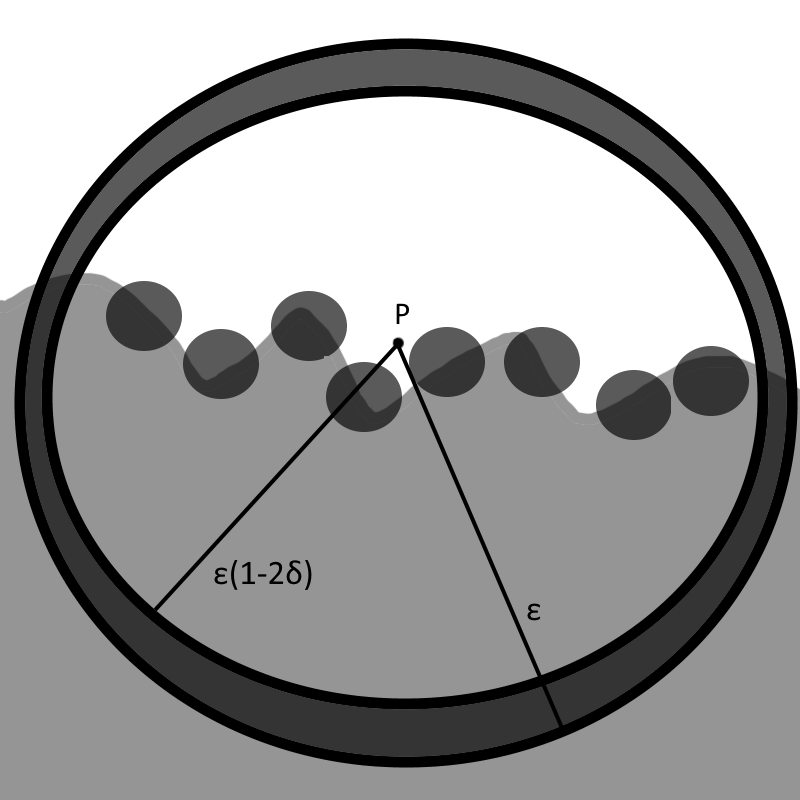
\includegraphics[width=0.4\textwidth]{covering lemma}
\end{figure}

Since $du$ is supported in $\bigcup_n 2V_n$,
$$|d\varphi|(x) - \partial_0\varphi(x) = \int_{B_\varepsilon} \chi_\varepsilon(x - \cdot)(|du| - \partial_0 u) \leq \sum_{n=0}^N \int_{2V_n} \chi_\varepsilon(x - \cdot)(|du| - \partial_0 u).$$
So, we shall show
\begin{equation}\label{bound on balls}
\int_{2V_n} \chi_\varepsilon(x - \cdot)(|du| - \partial_0u) \lesssim_{g, p, P} \gamma^{O(1)} \int_{V_n} \chi_\varepsilon(x - \cdot)|du|
\end{equation}
for $n \geq 1$ and
\begin{equation}\label{bound on balls 2}
\int_{V_0} \chi_\varepsilon(x - \cdot)(|du| - \partial_0u) \lesssim_{g, p, P} \gamma^{O(1)} \int_{B_\varepsilon} \chi_\varepsilon(x - \cdot)|du|,
\end{equation}
provided that $x = (r, \Theta)$ satisfies $r < \sigma$ and $\varphi \in (o(\gamma), 1 - o(\gamma))$.
If (\ref{bound on balls}, \ref{bound on balls 2}) are true, then since the balls $V_n$ are disjoint, we can sum over $n$ to obtain
\begin{equation}\label{claim on main mollifier lemma 2}|d\varphi|(x) - \partial_0\varphi(x) \lesssim_{g, p, P} \gamma^{O(1)} \int_{B_\varepsilon} \chi_\varepsilon(x - \cdot)|du| \leq \gamma^{O(1)} |d\varphi|(x),
\end{equation}
which implies (\ref{claim on main mollifier lemma}). Thus we may fix
$$x \in \partial^* U \cap \{r < \sigma\} \cap \{\varphi \in (f(\gamma), 1 - f(\gamma)),$$
and choose $\gamma$ so small that (\ref{claim on main mollifier lemma 2}) simplifies to $\partial_0 \varphi(x) \gtrsim |d\varphi(x)|$.
Thus, in particular,
$$\partial_0 \varphi(x) \gtrsim \int_{B_\varepsilon} \chi_\varepsilon(x - \cdot) |du| > 0.$$
By Lemma \ref{mollifier props}, $d\varphi$ is continuous, so the level sets of $\varphi$ must be $C^1$.
\end{proof}

\begin{proof}[Proof of (\ref{bound on balls})]
By (\ref{approximation of mollifier 2}), if $\gamma$ is small enough depending on $g$\footnote{One might worry that we frequently rescale $g$ in this paper.
However, in all of our rescalings, the curvature tensor remains in some bounded set, so these rescalings will never send $\gamma$ to $0$.}, then for every $y \in 2V_n$,
\begin{align*}
\int_{2V_n} \chi_\varepsilon(x - \cdot)(|du| - \partial_0u) &\lesssim F_n(x) \int_{2V_n} |du| - \partial_0u ~\vol, \\
F_n(x) &:= \frac{1}{\varepsilon^d}\left(1 - \frac{d(x, Q_n)}{\varepsilon}\right).
\end{align*}
If $\gamma$ is chosen small enough, then $\sigma > 2\delta\varepsilon$ and so if we set $W_n = B(Q_n, \sigma)$ and apply Proposition \ref{Monotonicity Formula},
\begin{align*}
\int_{2V_n}|du| - \partial_0u ~\vol &\leq
B \left[\sigma^{1 - d}\int_{W_n} |du| - \partial_0u ~\vol + \sigma^{1 - d}\int_{W_n} \partial_0u ~\vol - (2\delta\varepsilon)^{1 - d}\int_{2V_n} \partial_0u ~\vol \right],\\
B &:= e^{O(1)(\sigma^2 - 4\delta^2\varepsilon^2)}(2\delta\varepsilon)^{d - 1}.
\end{align*}
From Taylor's theorem and the fact that $\sigma > 2\delta\varepsilon$,
\begin{align*}
B \lesssim \delta^{d - 1} \varepsilon^{d - 1} + \sigma^2 \delta^{d - 1} \varepsilon^{d - 1} \lesssim \delta^{d - 1} \varepsilon^{d - 1}
\end{align*}
if $\gamma$ is small.
By (\ref{hypothesis on main mollifier lemma}),
$$\sigma^{1 - d}\int_{W_n} |du| - \partial_0u ~\vol \leq \gamma^{\frac{1 - d}{2(d - 1)} + 1} = \gamma^{1/2}.$$
By Proposition \ref{Monotonicity Formula},
\begin{align*}
\sigma^{1 - d}\int_{W_n} \partial_0u ~\vol - (2\delta\varepsilon)^{1 - d}\int_{2V_n} \partial_0u ~\vol &\lesssim (1 + \alpha)\sqrt{\sigma^{1 - d} \int_{W_n} |du| ~\vol - (2\delta\varepsilon)^{1 - d} \int_{2V_n} |du| ~\vol},\\
&\alpha := (d - 1)\log \frac{\sigma}{2\delta\varepsilon}.
\end{align*}
By Lemma \ref{scalar curvature monotonicity},
$$\sigma^{1 - d} \int_{W_n} \partial_0 u ~\vol - (2\delta\varepsilon)^{1 - d} \int_{2V_n} |du| ~\vol \leq (\sigma^2 -4\delta^2\varepsilon^2) \kappa(Q_n) + O(\sigma^4) \lesssim \sigma^2,$$
so by (\ref{hypothesis on main mollifier lemma}),
\begin{align*}
\sigma^{1 - d} \int_{W_n} |du| ~\vol - (2\delta\varepsilon)^{1 - d} \int_{2V_n} |du| ~\vol &= \sigma^{1 - d} \int_{W_n} |du| - \partial_0u ~\vol \\
&\qquad + \sigma^{1 - d} \int_{W_n} \partial_0u ~\vol - (2\delta\varepsilon)^{d - 1} \int_{W_n} |du| ~\vol \\
&\leq \gamma + O(\sigma^2) \lesssim \sigma^2.
\end{align*}
It follows from the definitions that
$$(1 + \alpha)\sigma \lesssim -\gamma^{1/2(d - 1)} \log \gamma \lesssim \gamma^{1/3(d - 1)}.$$
Summing up everything in this step of the proof thus far,
\begin{equation}\label{big bound 1}
\int_{2V_n} \chi_\varepsilon(x - \cdot)(|du| - \partial_0u) ~\vol \lesssim \delta^{d - 1} \varepsilon^{d - 1} F_n(x) \gamma^{1/3(d - 1)}.
\end{equation}
Since $U$ has least perimeter, Proposition \ref{doubling dimension} implies that
$$\delta^{d - 1} \varepsilon^{d - 1} \lesssim \int_{V_n} |du| ~\vol,$$
so by (\ref{approximation of mollifier 2}, \ref{big bound 1}),
\begin{align*}
\int_{2V_n} \chi_\varepsilon(x - \cdot)(|du| - \partial_0u) ~\vol
&\lesssim \gamma^{1/3(d - 1)} \int_{V_n} \chi_\varepsilon(x - \cdot)|du|.
\qedhere \end{align*}
\end{proof}

\begin{proof}[Proof of (\ref{bound on balls 2})]
From (\ref{approximation of mollifier 2}) it easily follows that for $y \in V_0$, $\chi_\varepsilon(x - y)/\vol(x - y) \lesssim \frac{\delta}{\varepsilon^d}$,
whence, by minimality of $\partial^* U$,
\begin{align*}
\int_{V_0} \chi_\varepsilon(x - \cdot)(|du| - \partial_0u) &\lesssim \frac{\delta}{\varepsilon^d} \int_{B_\varepsilon} |du| ~\vol \lesssim \frac{\delta}{\varepsilon^d} |\partial B_\varepsilon| \lesssim \frac{\delta}{\varepsilon}.
\end{align*}
By Lemma \ref{Giusti71}, there exists $c > 0$ such that if $\varphi \in (c\gamma^2, 1 - c\gamma^2)$, then $d(x, \partial U) < \varepsilon(1 - \gamma)$, so in particular we can find $Q \in \partial^* U$ such that $d(x, Q) < \varepsilon(1 - \gamma)$.
If $d(y, Q) < \gamma\varepsilon/2$, then
$$d(x, y) \leq \varepsilon - \gamma\varepsilon + \frac{\gamma\varepsilon}{2} \leq \varepsilon - \frac{\gamma\varepsilon}{2},$$
so by (\ref{approximation of mollifier 2}), $\chi_\varepsilon(x - y)/\vol(x - y) \gtrsim \frac{\gamma}{\varepsilon^d}$
for every $y \in B(Q, \gamma\varepsilon/2)$.
In particular, since $\delta = \gamma^d$, minimality of $\partial^* U$ gives
\begin{align*}
\int_{V_0} \chi_\varepsilon(x - \cdot)(|du| - \partial_0u) &\lesssim \frac{\delta}{\gamma^{d - 1}} \frac{\gamma^{d - 1}}{\varepsilon}\\
&\lesssim \gamma |\partial B(Q, \gamma\varepsilon/2)| \int_{B(Q, \gamma\varepsilon/2)} \chi_\varepsilon(x - \cdot) \\
&\lesssim \gamma \int_{B(Q, \gamma\varepsilon/2)} \chi_\varepsilon(x - \cdot) |du|\\
&\lesssim \gamma \int_{B_\varepsilon} \chi_\varepsilon(x - \cdot) |du|. \qedhere
\end{align*}
\end{proof}

%%%%%%%%%%%%%%%%%%%%%%%%%%%%%%%%%%%%%%%%%%%%%%%%%%%%%

\subsection{Proof of Proposition \ref{mollifier proposition}}
Select $t \in (0, 1)$ uniformly at random.
Let $w_n = (u_n)_{\gamma_n^4}$, let $c$ be the constant given by Lemma \ref{main mollifier lemma}, and let $a_n = c\gamma_n$, $b_n = 1 - c\gamma_n$.
0By Proposition \ref{Coarea2},
$$\int_{B_t} |dw_n| ~\vol = \int_0^1 |\partial^* \{w_n > y\} \cap B_t| ~dy \geq \int_{a_n}^{b_n} |\partial^* \{w_n > y\} \cap B_t| ~dy.$$
By the mean value theorem, there exists $y_n \in (a_n, b_n)$ such that
\begin{equation}\label{MVT mollifier}
|\partial^* \{w_n > y_n\} \cap B_t| \leq \frac{1}{b_n - a_n} \int_{B_t} |dw_n| ~\vol.
\end{equation}
If set $V_n = \{w_n > y_n\}$, $v_n = 1_{V_n}$, then $V_n$ has $C^1$ boundary in $B_t$ by definition of $a_n, b_n$, and from (\ref{claim on main mollifier lemma}), the locally uniform convergence (\ref{mollifier prop4}) holds.

So it remains to show that (\ref{mollifier prop1}--\ref{mollifier prop3}) hold almost surely.
Towards this end we will later show that
\begin{align}
|\partial V_n \cap B_t| &\leq |\partial^* U_n \cap B_t| + o(\gamma_n), \label{approximation of surface area} \\
\int_{\partial B_t} |u_n - v_n| ~\vol_{\partial B_t} &\lesssim \gamma_n^2. \label{approximation of volume}
\end{align}
If (\ref{approximation of surface area}, \ref{approximation of volume}) are true,
then by (\ref{a priori estimate 3}, \ref{approximation of volume}),
$$|\partial^* U_n \cap B_t| \leq |\partial V_n \cap B_t| + o(\gamma_n)$$
so by (\ref{approximation of surface area}), (\ref{mollifier prop2}) holds.
From an integration by parts using the fact that $\partial_j$ is a component of a quasieuclidean frame, and (\ref{approximation of volume}),
\begin{align*}
\left|\int_\Omega \partial_j(u_j - v_j) ~\vol\right|
&\leq \left|\int_{\partial \Omega} (u_j - v_j)g(\partial_j, \normal) ~\vol_{\partial \Omega}\right| \\
&\lesssim \int_{\partial \Omega} |u_j - v_j| ~\vol_{\partial \Omega} \lesssim \gamma_n^2
\end{align*}
which gives (\ref{mollifier prop3}).
By the fact that $U_n$ has least perimeter, and (\ref{a priori estimate 1}, \ref{mollifier prop2}),
\begin{align*}
|\partial V_n \cap B_t| &\leq |\partial U_n \cap B_t| + o(\gamma_n) \\
&= \eta(U_n, B_t) + o(\gamma_n)\\
&\leq \eta(V_n, B_t) + \int_{\partial B_t} |u_n - v_n| ~\vol_{\partial B_t} + o(\gamma_n),
\end{align*}
so by (\ref{approximation of volume}), (\ref{mollifier prop1}) holds.

%%%%%%%%%%%%%%%%%%%%%%%%%%%%%%%%%%%%%%%%%%%%%%%%%%%%%%%%%%%%%%%%

\begin{proof}[Proof of (\ref{approximation of surface area})]
By Lemma \ref{Giusti72}, one has
\begin{equation}\label{Giusti 720a}
\limsup_{n \to \infty} \int_{B_t} |du_n| - |dw_n| ~\vol \leq \limsup_{n \to \infty} \int_{B_{t + \gamma_n^4} \setminus B_t} |du_n| ~\vol.
\end{equation}
If we define $\mu = \sum_n \gamma_n|du_n| ~\vol$, then $\mu(B_1) < \infty$, since $(\gamma_n) \in \ell^1$ and $|\partial^* U_n \cap B_1|$ is uniformly bounded (c.f. Proposition \ref{doubling dimension}).
The hypotheses of \cite[(7.20)]{Giusti77} are (\ref{Giusti 720a}) and the fact that $\mu$ is a finite Borel measure on $B_1$, and the conclusion is that almost surely,
\begin{equation}\label{Giusti 720b}
\limsup_{n \to \infty} \gamma_n^{-2} \int_{B_t} |dw_n| - |du_n| ~\vol \leq 0.
\end{equation}
From (\ref{MVT mollifier}, \ref{Giusti 720b}), one has (\ref{approximation of surface area}).
\end{proof}

\begin{proof}[Proof of (\ref{approximation of volume})]
Let
$$f_n(t) = \gamma_n^{-4} \int_{B_t} |u_n - w_n| ~\vol.$$
By Lemma \ref{Giusti72} and the fact that $U_j$ has least perimeter in $B_1$,
$$\limsup_{n \to \infty} f_n(t) \leq \limsup_{n \to \infty} \int_{B_1} |du_n| ~\vol \leq |\partial B_1|.$$
Moreover, $f_n$ is monotone.
This implies that almost surely, $f_n'(t)$ is uniformly bounded in $n$.
But
$$f_n'(t) = \gamma_n^{-4} \int_{\partial B_t} |u_n - w_n| ~\vol_{\partial B_t},$$
so
\begin{equation}\label{mollify cubic gamma}
\int_{\partial B_t} |u_n - w_n| ~\vol_{\partial B_t} \lesssim \gamma_n^4.
\end{equation}
We now set $z_n = \min(y_n, 1 - y_n)$ and estimate
\begin{align*}
\int_{\partial B_t} |u_n - v_n| ~\vol_{\partial B_t} &= |\partial B_t \cap U_n \Delta V_n| \\
&= |\partial B_t \cap V_n \setminus U_n| + |\partial B_t \cap U_n \setminus V_n| \\
&\leq \frac{y_n}{z_n} |\partial B_t \cap V_n \setminus U_n| + \frac{1 - y_n}{z_n} |\partial B_t \cap U_n \setminus V_n|.
\end{align*}
From definition of $V_n$, $w_n - u_n > y_n$ on $V_n \setminus U_n$ and $u_n - w_n > 1 - y_n$ on $U_n \setminus V_n$, so
\begin{align*}
\int_{\partial B_t} |u_n - v_n| ~\vol_{\partial B_t} &\leq z_n^{-1} \int_{\partial B_t \cap U_n \setminus V_n} |u_n - w_n| ~\vol_{\partial B_t} + z_n^{-1}\int_{\partial B_t \cap V_n \setminus U_n} |u_n - w_n| ~\vol_{\partial B_t} \\
&\leq z_n^{-1} \int_{\partial B_t} |u_n - w_n| ~\vol_{\partial B_t}.
\end{align*}
But
$$z_n^{-1} \leq \max(y_n^{-1}, (1 - y_n)^{-1}) \leq \max(a_n^{-1}, b_n^{-1}) \lesssim \gamma_n^{-2}$$
whence
$$\int_{\partial B_t} |u_n - v_n| ~\vol_{\partial B_t} \lesssim \gamma_n^{-2} \int_{\partial B_t} |u_n - w_n| ~\vol_{\partial B_t},$$
so by (\ref{mollify cubic gamma}), (\ref{approximation of volume}) holds.
\end{proof}




%%%%%%%%%%%%%%%%%%%%%%%%%%%%%%%%%%%%%%%%%%%%%%%%%%%%%%

\section{de Giorgi lemma}\label{DeGiorgiSection}
TODO: Put all this in context...

\subsection{Multilinear computations}
Before formulating de Giorgi's lemma we begin by carrying out some computations in multilinear algebra which we will use to estimate the surface area Lagrangian.
We remind the reader of our conventions for Einstein summation, Notation \ref{EinsteinNotation}.

Suppose that we are given a $d$-dimensional oriented real Hilbert space $(\Hilb, g)$, and an oriented basis $(\partial_0, \dots, \partial_{d - 1})$ which may not be orthonormal but which satisfies for every $i$
\begin{equation}\label{0th coordinate orthogonal}
g_{0i} = 0
\end{equation}
where $g_{\mu\nu} = g(\partial_\mu, \partial_\nu)$.
We write $g_{\hat 0 \hat 0}$ for the inner product on the span $\Hilb_0^\perp$ of $\partial_1, \dots, \partial_{d - 1}$ defined by $(g_{\hat 0 \hat 0})_{ij} = g_{ij}$.
We as usual write $g^{\mu\nu}$, $(g^{\hat 0 \hat 0})^{ij}$ for the components of the dual metric, and $\delta_\mu^\nu$ for the components of the identity matrix.

\begin{definition}
The \dfn{Gramian matrix} of $v_1, \dots, v_{d - 1}$ is
$$\Gram(v_1, \dots, v_{d - 1})_{ij} = g_{\mu \nu} v_i^\mu v_j^\nu.$$
The \dfn{cross product} $v_1 \times \cdots \times v_{d - 1}$ of vectors $v_1, \dots, v_{d - 1} \in \Hilb$ is defined to be the vector $v_0$
such that:
\begin{enumerate}
\item $g(v_0, v_i) = 0$,
\item $((-1)^{d - 1} v_0, v_1, \dots, v_{d - 1})$ is positively oriented, and
\item the length is
$$|v_0|_g^2 = |\det \Gram(v_1, \dots, v_{d - 1})|.$$
\end{enumerate}
\end{definition}

Here the orientation convention is chosen so that if $\partial_0, \dots, \partial_{d - 1}$ is an orthonormal basis, thus $g_{\mu\nu} = \delta_{\mu\nu}$, then the cross product is computed by the formal determinant
\begin{equation}\label{formal determinant}
v_1 \times \cdots \times v_{d - 1} = \begin{vmatrix}\partial_0 & \cdots & \partial_{d - 1} \\
v_1^0 & \cdots & v_1^{d - 1}\\
& \vdots \\
v_{d - 1}^0 & \cdots & v_{d - 1}^{d - 1}\end{vmatrix}
\end{equation}
which of course agrees with the orientation convention of the cross product on $\RR^3$.

\begin{lemma} \label{cross product formula}
Suppose that $\phi_1, \dots, \phi_{d - 1} \in \Hilb$ satisfy $\phi_i^0 = \psi_i$, $\phi_i^j = \delta_i^j$ for some $\psi \in (\Hilb_0^\perp)'$.
Let $h_{ij} = (g_{00})^{-1} g_{ij}$, and let $\normal \in \Hilb'$ be the unit covector which annihilates $\phi_1, \dots, \phi_{d - 1}$ with $((-1)^{d - 1}\normal^\sharp, \phi_1, \dots, \phi_{d - 1})$ positively oriented.
Then
\begin{align}
|\det \Gram(\phi_1, \dots, \phi_{d - 1})| &= (g_{00})^{d - 1} (1 + |\psi|_{h^{-1}}^2) \det h, \label{WeinsteinAronszajn} \\
(\phi_1 \times \cdots \times \phi_{d - 1})^\mu &= (g_{00})^{d/2} g^{\mu \nu}(\delta_\nu^0 - \delta^i_\nu \psi_i) \sqrt{\det h}, \label{CrossProduct} \\
\normal_\mu &= \sqrt{\frac{g_{00}}{1 + |\psi|_{h^{-1}}^2}} (\delta^0_\mu - \delta^i_\mu \psi_i) \label{conormal crossproduct}.
\end{align}
\end{lemma}
\begin{proof}
We begin by computing
$$\Gram(\phi_1, \dots, \phi_{d - 1})_{ij} = g_{\mu \nu} \phi_i^\mu \phi_j^\nu = g_{00} \psi_i \psi_j + g_{ij}$$
which are the components of $g_{00}\psi \otimes \psi + g_{\hat 0 \hat 0} \in (\Hilb_0^\perp \otimes \Hilb_0^\perp)'$.
By the Weinstein-Aronszajn theorem \cite{Tao13}, $\det(1 + h^{-1}(\psi \otimes \psi)) = 1 + |\psi|_{h^{-1}}^2$, so
\begin{align*}
\det(g_{00}\psi \otimes \psi + g_{\hat 0 \hat 0})
&= (g_{00})^{d - 1} \det(\psi \otimes \psi + h) = (g_{00})^{d - 1} \det(h^{-1}(\psi \otimes \psi) + 1) \det h \\
&= (g_{00})^{d - 1} (1 + |\psi|_{h^{-1}}^2) \det h.
\end{align*}
Since $h$ is a quadratic form of signature $(+, \cdots, +)$, its determinant is positive and so (\ref{WeinsteinAronszajn}) holds.

We begin the proof of (\ref{CrossProduct}) by checking orthogonality:
\begin{align*}
g_{\mu\nu} g^{\mu \lambda} (\delta^0_\lambda - \delta^i_\lambda \psi_i)(\delta^\nu_0 \psi_i + \delta^\nu_i)
&= \delta^\lambda_\nu (\delta^0_\lambda - \delta^i_\lambda \psi_i)(\delta^\nu_0 \psi_i + \delta_i^\nu)
= \psi_i - \psi_i = 0.
\end{align*}
To check orientation we may assume that $g_{\mu\nu} = \delta_{\mu\nu}$ in which case we just need to check agreement with (\ref{formal determinant}):
$$\begin{vmatrix} \partial_0 && \cdots && \partial_{d - 1} \\
\psi_1 & 1 & 0 & \cdots & 0 \\
\psi_2 & 0 & 1 & \cdots & 0\\
&& \vdots \\
\psi_{d - 1} & 0 & \cdots & 0 & 1
\end{vmatrix} = \partial_0 - \sum_i \psi_i \partial_i.$$
To see that its length is $\det \Gram(\phi_1, \dots, \phi_{d - 1})$ we compute
\begin{align*}
g_{\mu \nu} g^{\mu \lambda}(\delta^0_\lambda - \delta^i_\lambda \psi_i) g^{\nu \kappa}(\delta_\kappa^0 - \delta_\kappa^j \psi_j)
&= (\delta_\mu^0 - \delta_\nu^i \psi_i)(g^{0 \nu} - g^{j \nu} \psi_j)\\
&= g^{00} - g^{0j} \psi_j - g^{0i} \psi_i + g^{ij} \psi_i \psi_j.
\end{align*}
Recalling (\ref{0th coordinate orthogonal}) we can rewrite this as
$$g_{\mu \nu} g^{\mu \lambda}(\delta^0_\lambda - \delta^i_\lambda \psi_i) g^{\nu \kappa}(\delta_\kappa^0 - \delta_\kappa^j \psi_j) = (g_{00})^{-1} + (g_{\hat 0 \hat 0})^{-1}(\psi \otimes \psi).$$
But $g_{00} (g_{\hat 0 \hat 0})^{-1} = h^{-1}$ so we deduce from (\ref{WeinsteinAronszajn})
$$g_{\mu \nu} g^{\mu \lambda}(\delta^0_\lambda - \delta^i_\lambda \psi_i) g^{\nu \kappa}(\delta_\kappa^0 - \delta_\kappa^j \psi_j) = (g_{00})^{-1} (1 + |\psi|_{h^{-1}}^2)
= \frac{|\det \Gram(\phi_1, \dots, \phi_{d - 1})|}{(g_{00})^d \det h}$$
which gives (\ref{CrossProduct}).
From (\ref{WeinsteinAronszajn}, \ref{CrossProduct}), (\ref{conormal crossproduct}) is immediate.
\end{proof}

%%%%%%%%%%%%%%%%%%%%%%%%%%%%%%%%%%%%%%%%%%%%%%%%

\subsection{The Killing foliation}
In euclidean space, one can view a $C^1$ hypersurface as a graph using the usual coordinates, possibly up to a rotation.
We would like to view $C^1$ hypersurfaces in $M$ as graphs, and to do so in a way which is favorable for our later work, we will need assume that the coordinate system of $M$ is foliated by hypersurfaces which are all isometric to each other.

\begin{definition}\label{Killing setup}
Let $H$ be a hypersurface in some open subset of $M$ which is normal to a Killing field $X$, and $P \in H$.
We associate the following data to $(H, X, P)$:
\begin{enumerate}
\item The \dfn{Killing weight}: A scalar field $\lambda = g(X, X)^{(d - 1)/2}$ on $H$.
\item The \dfn{weighted metric}: A metric $h(v, w) = g(X, X)^{-1} g(v, w)$ on $H$.
\item The \dfn{Killing foliation}: An open immersion $\chi: H \times I \to M$ defined by making $\chi(x, \cdot)$ the integral curve of $X$ centered on $x \in H$.
\item The \dfn{area Lagrangian}: A family of $d-1$-forms on $H$ parametrized by $1$-forms $\psi$ on H, and defined by
\begin{equation}\label{area Lagrangian}
\Lagrange(\psi) = \lambda \sqrt{1 + |\psi|_{h^{-1}}^2} \vol_h.
\end{equation}
\end{enumerate}
\end{definition}

\begin{lemma}\label{Giusti46}
Let $U \subseteq M$ be a set of $C^1$ boundary, let $X$ be a vector field such that $(\normal_U, X) > 0$, and let $T > 0$.
If $x: [-T, T] \to M$ is an integral curve of $X$ such that $x(0) \in \partial U$, then for every $t \in (0, T)$, $x(t) \in U$ and $x(-t) \in U$.
\end{lemma}
\begin{proof}
The claimed assertions are all local, so we may assume that $M$ is diffeomorphic to an open subset of $\RR^d$.
By Proposition \ref{metric-independence theorem}, we may without loss of generality assume that $M$ is actually isometric to an open subset of $\RR^d$ with its usual metric, $X$ is a coordinate field on $\RR^d$, and $x$ is a line segment.
By taking a compact exhaustion of $M$ and applying the fact that $\partial U$ is $C^1$, we may also assume that there exists $\delta > 0$ such that $(\normal_U, X) \geq \delta$ almost everywhere.
This reduces the claimed assertions to \cite[Lemma 4.6, Remark 4.7]{Giusti77}.
\end{proof}

\begin{lemma}\label{hopfKilling}
Assume that $M$ is a locally homogeneous Riemannian manifold.
Then for every pointed $C^1$ hypersurface $(N, P)$ in $M$ there exists a hypersurface $H \ni P$ in some neighborhood of $P$ and a Killing field $X$, of unit length at $P$, such that $H$ is tangent to $N$ at $P$ and $H$ is normal to $X$, and for which $N$ is a graph in the following quantitative sense:

Let $\chi$ be the Killing foliation associated to $(H, X, P)$.
Then there exists a $C^1$ function $\omega: H \to \RR$ such that in some neighborhood $M'$ of $P$,
\begin{align}
N \cap M' &= \{\chi(x, \omega(x)): x \in H \cap M'\} \label{N is a graph}\\
||d\omega||_{L^\infty(M')} &\lesssim \sup \frac{1}{(\normal, X)} < \infty \label{derivative bounds}
\end{align}
where $\normal = \normal_N$ is taken so that $\normal^\sharp$ and $X$ both point into the same open set.
\end{lemma}
\begin{proof}
Let $X$ be an infinitesimal generator of the local Lie group of $M$ in a neighborhood of $P$, chosen to be normal to $N$ at $P$ and rescaled so that $g(X, X) = 1$ at $P$.
Let $E = X^\perp$ be its orthocomplement bundle. Then $E$ is involutive, so by the Frobenius theorem, there exists $H$ which is normal to $X$ and $P \in H$.
Since $X$ is normal to $H$ and is normal to $N$ at $P$, $H$ is tangent to $N$ at $P$.

Since $X$ is normal to $H$, $\normal = \normal_N$ satisfies $\inf (\normal, X) > 0$ if we select $M'$ small enough, say $(\normal, X) \geq \delta > 0$.
The existence of a function $\omega$ which satisfies (\ref{N is a graph}) is now clear from the implicit function theorem.
Given a unit vector field $Y$, we can estimate
\begin{align*}
(\normal, Y)
&\geq (\normal, X) \frac{g(Y, X)}{g(X, X)} - \sqrt{1 - \frac{(\normal, X)^2}{g(X, X)^2}}\sqrt{1 - \frac{g(Y, X)^2}{g(X, X)^2}}\\
&\geq \delta \frac{g(Y, X)}{g(X, X)} - \sqrt{1 - \frac{\delta^2}{g(X, X)^2}} \sqrt{1 - \frac{g(Y, X)^2}{g(X, X)^2}}
\end{align*}
and hence if
\begin{equation}\label{estimate on vector field}
\frac{g(Y, X)}{g(X, X)} \left(1 - \frac{g(Y, X)^2}{g(X, X)^2}\right)^{-1/2} > \frac{\sqrt{1 - \delta^2 g(X, X)^{-2}}}{\delta},
\end{equation}
on $N$, Lemma \ref{Giusti46} implies that for every integral curve $y$ of $Y$ with $y(0) = (x, \omega(x))$, $x \in H$, then $y(t) = (x', \omega(x'))$ implies $x' = x$, $t = 0$.
In particular this is the case when $y$ is a geodesic through $(x, \omega(x))$ for which $Y = y'(x, \omega(x))$ satisfies (\ref{estimate on vector field}).

\begin{figure}[h]
\caption{The geodesic (blue) passes through $N$ (pink) repeatedly, and therefore must miss the cone of integral curves which satisfy (\ref{estimate on vector field}).}
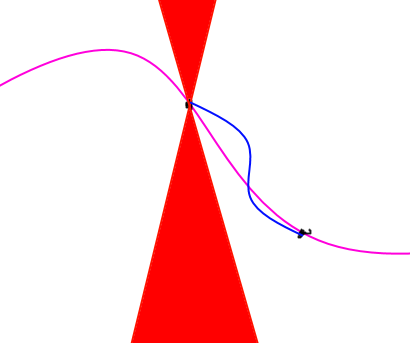
\includegraphics[width=0.4\textwidth]{graph_cone}
\end{figure}

If $x'$ is close to $x$, then there must be a geodesic $y$ connecting $(x, \omega(x))$ to $(x', \omega(x'))$ and such a geodesic must satisfy the negation of (\ref{estimate on vector field}).
In that case we therefore have
$$\frac{d(\omega(x), \omega(x'))}{d(x, x')} \lesssim g(Y, X) \lesssim \delta^{-1}$$
since $y$ is a geodesic and the claim follows when we take $x' \to 0$.
\end{proof}

\begin{lemma}\label{volume form is Lagrangian}
Let $N$ be a $C^1$ hypersurface in $M$, such that there exists a Killing foliation $\chi$ associated to a triple $(H, \partial_0, P)$ and a $C^1$ function $\omega$ whose graph is $N$, c.f. (\ref{N is a graph}).
Let $\vol_N$ be the volume form induced on $N$ by $g$, and let $\varphi(x) = (x, \omega(x))$ be the induced diffeomorphism $H \to N$.
Then:
\begin{enumerate}
\item The area Lagrangian $\Lagrange$ associated to $(H, X, P)$ satisfies
\begin{equation}\label{volume form pullback}
\varphi^* \vol_N = \Lagrange(d\omega).
\end{equation}
\item Let $\partial_1, \dots, \partial_{d - 1}$ be (the translates by $\partial_0$ of) a quasieuclidean frame on $H$ and let $S$ be a small open subset of $M$. Then
$$\int_S u_{,\mu} ~\vol = \int_{\varphi^{-1}(S \cap N)} \sqrt{g_{00}} (\delta_\mu^0 - \delta^i_\mu \omega_{,i}) ~\vol_H.$$
\end{enumerate}
\end{lemma}
\begin{proof}
Since $\partial_0$ is a Killing field,
\begin{equation}\label{preservation of scalar field}
0 = \delta^\lambda_0 g_{\mu \nu,\lambda} + \delta^\lambda_{0,\mu} g_{\nu\lambda} + \delta^\lambda_{0,\nu} g_{\mu \lambda} = g_{\mu\nu,0},
\end{equation}
so the scalar field $g_{\mu\nu}$ is preserved by $\varphi^*$.
Moreover, since $\partial_0$ is assumed normal to $H$, $g_{0i} = 0$.
If we write $\slashed g$ for the metric induced by $g$ on $N$, then
$$\varphi^* \vol_N = \varphi^* \sqrt{\det \slashed g} ~dx = \sqrt{\varphi^* \det \slashed g} ~dx.$$
From Lemma \ref{cross product formula} with $\psi = d\omega$, we obtain
\begin{align*}
\varphi^* \vol_N &= \lambda\sqrt{1 + |d\omega|_{h^{-1}}^2} \sqrt{\det h} ~dx = \Lagrange(d\omega)
\end{align*}
which proves (\ref{volume form pullback}).
Using (\ref{volume form pullback}, \ref{preservation of scalar field}) and the fact that $N$ is $C^1$, we also compute
\begin{align*}
\int_S u_{,\mu} ~\vol &= \int_{S \cap N} \normal_\mu ~\vol_N \\
&= \int_{\varphi^{-1}(S \cap N)} \sqrt{\frac{g_{00}}{1 + |\psi|_{h^{-1}}^2}} (\delta_\mu^0 - \delta_\mu^i \omega_{,i})\Lagrange(d\omega) \\
&= \int_{\varphi^{-1}(S \cap N)} (g_{00})^{d/2} (\delta_\mu^0 - \delta_\mu^i \omega_{,i}) \vol_h \\
&= \int_{\varphi^{-1}(S \cap N)} \sqrt{g_{00}} (\delta_\mu^0 - \delta_\mu^i \omega_{,i}) ~\vol_H \qedhere.
\end{align*}
\end{proof}

%%%%%%%%%%%%%%%%%%%%%%%%%%%%%%%%%%%%%%%%%%%%%

\subsection{Deforming the mean-value property}
Our next task is to show that the area Lagrangian (\ref{area Lagrangian}) satisfies an approximate mean-value property, which gives an improvement on \cite[Teorema 4.3]{Miranda66}.

\begin{notation}
Let $(H, h, P)$ be a pointed Riemannian manifold of dimension $d - 1$.
We define a metric $\tilde h$ with vanishing curvature by considering normal coordinates $x_1, \dots, x_{d - 1}$ with respect to $h$ and setting $\tilde h_{ij} = \delta_{ij}$, thus
$$h_{ij} = \tilde h_{ij} + O(x^2)$$
where the implied constant depends continuously on $h$ and its derivatives at $P$.
We then define the $\tilde h$-Dirichlet energy
$$\DirL(\psi) = \frac{\tilde h^{ij} \psi_i \psi_j}{2}\vol_{\tilde h}.$$
Let $B_r$ denote a ball centered on $P$ in the euclidean space $(H, \tilde h)$, not in $M$.
Let $A(r)f$ denote the $\tilde h$-mean of $f$ over $B_r$.
Note that we can take means of $1$-forms as well as functions, since $\tilde h$ is flat.
\end{notation}

\begin{lemma}\label{Taylor lemma}
Let $(H, h, P)$ be a pointed Riemannian manifold of dimension $d - 1$, let $\lambda$ be a scalar field on $H$, let $\Lagrange$ satisfy (\ref{area Lagrangian}), and suppose that there exists $c \in (0, 1)$ such that for every $1$-form $\psi$,
\begin{align}
1 - c \leq |\lambda|, g_{00} \leq 1 + c, \label{estimate on Killing weight} \\
1 - c \leq \frac{|\psi|^2_{h^{-1}}}{|\psi|^2_{\tilde h^{-1}}} \leq 1 + c, \label{estimate on normal coordinates}\\
1 - c \leq \sqrt{\frac{\det h}{\det \tilde h}} \leq 1 + c, \label{estimate on normal volume form}
\end{align}
If $p,q$ are $1$-form on $H$ such that $|q|^2_{h^{-1}} \lesssim 1$, then $\Lagrange(p) - \Lagrange(q)$ lies in the closed interval
$$\left[\frac{1 - O(c)}{\Lagrange(q)}(\DirL(p) - \DirL(q)) - O(\DirL(p) - \DirL(q))^2, (1 + O(c))(\DirL(p) - \DirL(q))\right]$$
where all implied constants are absolute.
\end{lemma}
\begin{proof}
Let $\DirL_h(Y) = \sqrt{1 + h_{ij} Y^i Y^j}/2 ~\vol_h$ be the Dirichlet energy with respect to $h$.
Applying (\ref{estimate on normal coordinates}, \ref{estimate on normal volume form}),
\begin{equation}\label{estimate on normal coordinates 2}
1 - O(c) \leq \frac{\DirL(p) - \DirL(q)}{\DirL_h(p) - \DirL_h(q)} \leq 1 + O(c).
\end{equation}
By Taylor's theorem, there exists $\xi \geq 0$ between $|p|$ and $|q|$ such that
\begin{align*}
\lambda^{-1}(\Lagrange(p) - \Lagrange(q)) &= \sqrt{1 + |p|^2} - \sqrt{1 + |q|^2}\\
&= \frac{|p|^2 - |q|^2}{2 \sqrt{1 + |q|^2}} - \frac{(|p|^2 - |q|^2)^2}{8(1 + \xi^2)^{3/2}} \\
&= \frac{\DirL_h(p) - \DirL_h(q)}{\sqrt{1 + |q|^2}} - \frac{(\DirL_h(p) - \DirL_h(q))^2}{2(1 + \xi^2)^{3/2}}.
\end{align*}
Since $|q|^2 \geq 0$ and the second term is nonpositive, it follows from (\ref{estimate on Killing weight}, \ref{estimate on normal coordinates 2}) that
$$\Lagrange(p) - \Lagrange(q) \leq (1 + c)(\DirL_h(p) - \DirL_h(q)) \leq (1 + O(c))(\DirL(p) - \DirL(q)).$$
If $|q|^2_h$ is small enough,
$$2\Lagrange(q) \leq 8 \leq 8(1 + \xi^2)^{3/2},$$
whence
\begin{align*}
\frac{(1 + c)^{-1}(\DirL(p) - \DirL(q))}{\Lagrange(q)} - \frac{2(1 + c)^{-2}(\DirL(p) - \DirL(q))^2}{\Lagrange(q)} &\leq \Lagrange(p) - \Lagrange(q).
\end{align*}
Another application of (\ref{estimate on normal coordinates 2}) completes the proof.
\end{proof}

\begin{lemma}
For every $c \in (0, 1)$ there exists $\rho^* = \rho^*(c, g, P) > 0$ which depends continuously on $P$ and with the following property.

Let $H$ be a hypersurface which is normal to a Killing field, and for which $\chi,\Lagrange$ are given by Definition \ref{Killing setup}.
Let $\omega: H \to \RR$ be $C^1$, and suppose that $U \subseteq M$ is an open set such that
$$\partial U = \{\chi(x, \omega(x)): x \in H\}.$$
Then for every $\rho \in (0, \rho^*)$ and $\alpha, \kappa, \beta \in (0, 1)$ such that
\begin{align}
||d\omega||_{L^\infty(B_\rho)} &\leq \kappa, \label{Dirichlet small derivative}\\
\int_{B_\rho} \Lagrange(d\omega) - \Lagrange(A(\rho)d\omega) &\leq \beta, \label{Dirichlet close to mean} \\
\int_{B_\rho} \Lagrange(d\omega) &\leq \eta(U, \rho) + \beta \kappa, \label{Dirichlet close to minimal}
\end{align}
it follows that
\begin{equation}\label{Dirichlet gain}
\int_{B_{\alpha\rho}} \Lagrange(d\omega) - \Lagrange(A(\alpha\rho)d\omega) \leq (1 + O(c))\alpha^{d + 1}\beta + O(\beta \kappa^{1/2})
\end{equation}
where all implied constants are absolute.
\end{lemma}
The role of these parameters is as follows: we will take $\beta,\kappa \to 0$ in a proof by compactness and contradiction, and when we apply Proposition \ref{mollifier proposition}, we will take $\alpha \to 1/2$. One should think of $\beta$ as much smaller than $\kappa$, which in turn is much smaller than $c,\alpha,\rho^*$.
Indeed, $c$ will later be chosen absolutely, so $\rho^*$ only depends on $P,g$.
Once we have fixed $\rho^*$, we will iteratively halve the scale $\rho$ so that we can capitalize on (\ref{Dirichlet gain}).
\begin{proof}
Let $h,\lambda$ be as in Definition \ref{Killing setup}.
Then $\lambda(P) = 1$ and $\lambda$ depends only on $g,P$.
So we can use (\ref{Dirichlet small derivative}) and the fact that $\kappa < 1$ to select $\rho^*$ independently of $\omega$, so that such that
if $\rho < \rho^*$, then $\lambda$ is controlled by (\ref{estimate on Killing weight}),
$h$ is controlled by (\ref{estimate on normal coordinates}, \ref{estimate on normal volume form}), and
$$||d\omega||_{L^\infty(B_\rho)} \cdot |B_\rho| \lesssim 1.$$
Thus we will be able to apply Lemma \ref{Taylor lemma}.
Since $h$ is of the form $h(v, w) = g(X, X)^{-1} g(v, w)$ for a Killing field $X$, and the space of Killing fields defined near $P$ is finite-dimensional, $h$ and its derivatives are all controlled by $g,P$ and so $\rho^*$ is determined by $c,P,g$.

Let $u$ be the $\tilde h$-harmonic function on $B_\rho$ such that $u|\partial B_\rho = \omega|\partial B_\rho$.
By definition of $\eta(U, \rho)$ and (\ref{Dirichlet close to minimal}),
\begin{equation}\label{Dirichlet close to harmonic}
\int_{B_\rho} \Lagrange(d\omega) - \Lagrange(\nabla u) \leq \int_{B_\rho} \Lagrange(d\omega) - \eta(U, \rho) \leq \beta\kappa.
\end{equation}
We now proceed analogously to the proof of \cite[Lemma 4.2]{Miranda66}. By Lemma \ref{Taylor lemma},
\begin{align*}
\int_{B_{\alpha\rho}} \Lagrange(d\omega) - \Lagrange(A(\alpha\rho)d\omega) &\leq (1 + c)\int_{B_{\alpha\rho}} \DirL(d\omega) - \DirL(A(\alpha\rho)d\omega) \\
&= \frac{1 + c}{2} \int_{B_{\alpha\rho}} |d\omega|^2 - |A(\alpha\rho)d\omega|^2.
\end{align*}
Since $A(\alpha\rho)d\omega$ is the mean of $d\omega$, we have for every $\varepsilon > 0$
\begin{align*}
\int_{B_{\alpha\rho}} |d\omega|^2 - |A(\alpha\rho)d\omega|^2 &\leq \int_{B_{\alpha\rho}} (d\omega - A(\rho)d\omega)^2 ~dx \\
&\leq (1 + \varepsilon^{-1})\int_{B_\rho} |d\omega - \nabla u|^2 ~dx\\
&\qquad + (1 + \varepsilon) \int_{B_{\alpha\rho}} |\nabla u - A(\rho)d\omega|^2 ~dx\\
&=: O(\varepsilon^{-1})I + (1 + \varepsilon)J.
\end{align*}
To estimate $I$, we use the mean-value property, Lemma \ref{Taylor lemma}, and (\ref{Dirichlet close to harmonic}):
\begin{align*}
I &= \int_{B_\rho} |d\omega - \nabla u|^2 = \int_{B_\rho} |d\omega|^2 - |\nabla u|^2 \lesssim \int_{B_\rho} \Lagrange(d\omega) - \Lagrange(\nabla u) \leq \beta \kappa.
\end{align*}
To estimate $J$, we apply \cite[Lemma 4.1]{Miranda66}:
\begin{align*}
J &= \int_{B_\rho} |\nabla u|^2 - |A(\rho)d\omega|^2 = \int_{B_\rho} |\nabla u|^2 - |A(\rho)\nabla u|^2 \\
&\leq \alpha^{d + 1} \int_{B_\rho} |\nabla u|^2 - |A(\rho)\nabla u|^2 \leq \alpha^{d + 1} \int_{B_\rho} |d\omega|^2 - |A(\rho)d\omega|^2 \\
&\leq \alpha^{d + 1} \int_{B_\rho} |d\omega - A(\rho)d\omega|^2 ~dx \\
&\leq (1 + \varepsilon)\alpha^{d + 1} \int_{B_\rho} |d\omega - A(\rho)d\omega|^2  + O(\varepsilon^{-1})\int_{B_\rho} |d\omega - \nabla u|^2\\
&=: (1 + \varepsilon)\alpha^{d + 1}K + O(\varepsilon^{-1})I.
\end{align*}
We already estimated $I \lesssim \beta \kappa$, and now we estimate $K$: by Lemma \ref{Taylor lemma} and (\ref{Dirichlet small derivative}, \ref{Dirichlet close to mean}),
\begin{align*}
K &= \int_{B_\rho} |d\omega|^2 - |A(\rho)d\omega|^2\\
&\leq 2\int_{B_\rho} \DirL(d\omega) - \DirL(A(\rho)d\omega)\\
&\leq 2(1 + O(c))\int_{B_\rho} \Lagrange(d\omega) - \Lagrange(A(\rho)d\omega) + O(1) \int_{B_\rho} (\DirL(d\omega) - \DirL(A(\rho)d\omega))^2\\
&\leq 2(1 + O(c))\beta + O(1) ||d\omega||_{L^\infty(B_\rho)} \int_{B_\rho} \DirL(d\omega) - \DirL(A(\rho)d\omega) \\
&\leq 2\beta(1 + O(c + \kappa)).
\end{align*}
If we set $\varepsilon = \kappa^{1/2}$ then we conclude
\begin{align*}
\int_{B_{\alpha\rho}} \Lagrange(d\omega) - \Lagrange(A(\alpha\rho)d\omega)
&\leq (1 + O(c + \varepsilon)) \alpha^{d + 1}\beta + O(\beta \kappa \varepsilon^{-1})\\
&\leq (1 + O(c))\alpha^{d + 1} \beta + O(\beta \kappa^{1/2}). \qedhere
\end{align*}
\end{proof}

\subsection{$C^1$ case}
With the above setup, we now are ready to show the $C^1$ case of de Giorgi's lemma \cite[Teorema 4.4]{Miranda66}.
We again let $B_r$ denote a ball in $(M, g)$, not in some euclidean hypersurface $(H, h)$.

\begin{definition}
The (unnormalized) \dfn{excess} of a set $U$ of locally finite perimeter with respect to a quasieuclidean frame $(\partial_0, \dots, \partial_{d - 1})$ at $P$ is defined by
$$\Lambda_U(\rho) = \int_{B_\rho} |du| ~\vol - \sqrt{\sum_{j=0}^{d - 1} \int_{B_\rho} \partial_ju ~\vol}.$$
\end{definition}

\begin{lemma}\label{DGLC1}
Suppose that $M$ is a space form of dimension $2$ or nonpositive curvature, and let $(\partial_0, \dots, \partial_{d - 1})$ be a quasieuclidean frame defined near $P \in M$.
Let $(U_n)$ be a sequence of open sets with $C^1$ boundary.

Then for every $c \in (0, 1)$ there exists $\rho^* = \rho^*(c, g) > 0$ such that for every $\rho \in (0, \rho^*)$, if $\beta_n > 0$ satisfy
\begin{align}
\Lambda_{U_n}(\rho) &\leq \beta_n, \label{DGLC1 small excess}\\
\lim_{n \to \infty} ||g(\normal_{U_n}, \partial_0) - 1||_{L^\infty(B_\rho)} &= 0, \label{DGLC1 up normals}\\
|\partial U_n \cap B_\rho| &\leq \eta(U_n, B_\rho) + o(\beta_n), \label{DGLC1 almost minimal}
\end{align}
then
$$\limsup_{n \to \infty} \frac{\Lambda_{U_n}(\rho/2)}{\beta_n} \leq \frac{(1 + c)^2}{2^{d + 1}}.$$
\end{lemma}

\subsection{Mollification}
The same results as in the previous section hold without $N$ a $C^1$ hypersurface.
In particular:

\begin{proposition}\label{de Giorgi}
For every $c > 0$ there exists $\sigma > 0$ and $r > 0$ such that for every set $U$ of least perimeter, if
$\rho < r$ and
$$\Lambda(U, \rho) < \sigma \rho^{d - 1},$$
then
$$\Lambda(U, \rho/2) < \frac{(1 + c)^2}{2^d} \Lambda(U, \rho).$$
\end{proposition}

We now settle the choice of $c = c(d)$: we select $c$ so that that
$$\frac{(1 + c)^2}{2^d} < \lambda^{-d}$$
for some $\lambda \in (0, 1)$ such that
$$\frac{d - 1}{d} < \log_2 \lambda < 1.$$
By induction on Proposition \ref{de Giorgi}, there exists $\tau \in (0, 1)$ such that
\begin{equation}\label{inductive de Giorgi}
\Lambda(U, 2^{-n}) \lesssim 2^{-n(d - \tau)}.
\end{equation}

\subsection{Continuity of the conormal}
Let
$$\normal_s(P) = \frac{\int_{B_s(P)} du}{\int_{B_s(P)} |du|}.$$
Then $\normal_s \to \normal$ almost everywhere and $\normal_s$ is obviously continuous.
We want to get uniform convergence, thus we use the following lemma:

\begin{lemma}
Suppose that $0 < s < t < \rho$ are dyadic,
$$\Lambda(U, \rho) < \sigma \rho^{d - 1},$$
and $P \in \partial U$.
Then there exists $\delta > 0$ such that
$$|\normal_s(P) - \normal_t(P)| \lesssim t^\delta.$$
\end{lemma}
\begin{proof}
Write $s = 2^{-m}$, $t = 2^{-n}$ (so $m > n$), and set $v_k = \normal_{2^{-k}}(P)$, $M_k = \int_{B_{2^{-k}}} |du|$.
Then
$$|v_n - v_m|^2 \lesssim 1 - (v_n, v_m).$$
Gistui--Miranda show that
$$(1 - (v_n, v_m))M_m \leq 2M_n(1 - |v_n|) = 2\Lambda(U, t).$$
By (\ref{inductive de Giorgi}),
$$(1 - (v_n, v_m))M_m \lesssim 2^{-n(d - \tau)}$$
and hence, since $M_m \gtrsim 2^{-n(d - 1)}$, we conclude
\begin{align*}
|v_n - v_m|^2 &\lesssim 2^{-n(1 - \tau)} = t^{1 - \tau}. \qedhere
\end{align*}
\end{proof}

It follows from the above and the main theorem of Miranda66 that if
$$\Lambda(U, \rho) < \sigma \rho^{d - 1},$$
then $\normal$ is continuous in a neighborhood of $P$, and therefore $N$ is analytic.



%%%%%%%%%%%%%%%%%%%%%%%%%%%%%%%%%%%%%%%%%%%%%%%%%%%%%

\section{Proofs of main theorems}\label{proof of main thm}
We are finally ready to prove Theorems \ref{main thm}, \ref{main crly}, and \ref{main lma}.

\subsection{Regularity of minimal hypersurfaces}
We begin by proving Theorem \ref{main lma}.
Let $U$ be a set of least perimeter, and let $u$ be its indicator function.

We first may cover $M$ by normal coordinate charts $A_x$ centered on $x \in M$, selected so that $A_x$ is precompact in $M$.
In particular, if we fix a particular $x$, then the averaged $1$-forms $\int_V du ~\vol$ are well-defined for $V \subseteq A_x$, so the excesses $\Lambda(U, V)$ are well-defined.
We write $\Lambda_x$ for the excess as computed in $A_x$, and write $N^* = \partial^* U$.
Since $A_x$ is a precompact chart, we can select $\sigma_x$ to be the constant that appears in Proposition \ref{DGL}.

\begin{lemma}
For every $x \in N^*$ and sufficiently small $\rho > 0$ such that $B(x, \rho) \subseteq A_x$, there is an open set $x \in A_x' \subseteq A_x$ and $\delta > 0$ such that for every $t \in (0, \delta)$, $s \in (0, \rho)$, and $y \in A_x'$ such that $B(y, s) \subseteq A_x$,
\begin{equation}\label{basecase}\Lambda_x(U_t, B(y, s)) < \sigma_x s^d.\end{equation}
\end{lemma}
\begin{proof}
By Proposition \ref{blowup theorem}, there exists a half-space $C_x$ obtained as the blowup of $\exp_x^* U$\footnote{This is the only point in the argument when we use the fact that $d \leq 7$!}.
Since $C_x$ is a half-space and the coordinate chart $A_x$ is normal, $\Lambda_x((\exp_x)_* C_x, V) = 0$ whenever $V \subseteq A_x$.
In particular, if $V$ has no singularities with respect to the blowup sequence $(u_t)$,
$$\lim_{t \to 0} \Lambda_x(U_t, V) = \Lambda_x((\exp_x)_* C_x, V) = 0.$$
Here $U_t = (\exp_x)_* \{u_t = 1\}$ is the blowup of $U$.
So for every $\rho$ such that $B(x, \rho) \subseteq V$, there exists $\delta > 0$ such that if $t < \delta$,
$$\Lambda_x(U_t, B(x, \rho)) < \frac{\sigma_x}{2} \rho^d.$$
By continuity of measure, it follows that for every $y \in A_x$ close enough to $x$, and $0 < s < \rho$ such that $B(y, s) \subseteq A_x$, the claim holds.
\end{proof}

Fix $x \in N^*$, $t < \delta$, and let
$$\normal_s(y) = \frac{\int_{B(y, s)} du_t ~\vol}{\int_{B(y, s)} |du_t| ~\vol},$$
whenever $y \in A_x'$ and $B(y, s) \subseteq A_x$.
Then $\normal_s$ is continuous, since
$$\left|\int_{B(y_1, s)} du_t ~\vol - \int_{B(y_2, s)} du_t ~\vol\right| \leq \int_{B(y_1, s) \Delta B(y_2, s)} |du_t| ~\vol$$
where $\Delta$ denotes symmetric difference; the right-hand side vanishes as $y_2 \to y_1$ by continuity of measure.
We now show that $(\normal_s)$ is uniformly Cauchy as $s \to 0$.

\begin{lemma}
One has
$$|\normal_s(y) - \normal_r(y)| \lesssim_x \sqrt s$$
uniformly in $y \in A_x'$, whenever $0 < r < s < \rho$ and $B(y, s) \subseteq A_x$.
\end{lemma}
\begin{proof}
After throwing away a constant factor we may assume that $s = \rho/2^k$ for some $k$, and $r = \beta s$ for some $\beta \in (0, 1)$.
Since $|\normal_s(y)|,|\normal_r(y)| \leq 1$,
$$|\normal_s(y) - \normal_r(y)| \lesssim \sqrt{1 - (\normal_s(y), \normal_r(y))}.$$
Then (TODO: This seems dubious, check it)
\begin{align*}
(1 - (\normal_s(y), \normal_r(y)))  &\leq \frac{1}{|N^* \cap B(y, r)|} \int_{B(y, \beta \rho/2^k)} |du_t| - \left(\normal_s(y), \frac{du_t}{|du_t|}\right) |du_t| ~\vol\\
&\leq \frac{1}{|N^* \cap B(y, r)|} \int_{B(y, \rho/2^k)} |du_t| - \frac{(\normal_s(y), du_t)}{|du_t|} |du_t| ~\vol \\
&\leq \frac{1}{|N^* \cap B(y, r)|} \int_{B(y, \rho/2^k)} |du_t| - |\normal_s(y)|^2 |du_t| ~\vol\\
&\leq \frac{2}{|N^* \cap B(y, r)|} (1 - |\normal_s(y)|)\int_{B(y, \rho/2^k)} |du_t| ~\vol\\
&= 2\frac{\Lambda_x(U, B(y, s))}{|N^* \cap B(y, r)|}.
\end{align*}
By inducting on Proposition \ref{DGL} in $k$, the base case (\ref{basecase}), and Proposition \ref{doubling dimension},
\begin{align*}
\frac{\Lambda_x(U, B(y, s))}{|N^* \cap B(y, r)|} < 2^{-kd} \frac{\Lambda_x(U, B(y, \rho))}{r^{d - 1}} \lesssim s
\end{align*}
and therefore
\begin{align*}
|\normal_s(y) - \normal_r(y)| &\lesssim \sqrt{\frac{\Lambda_x(U, B(y, s))}{|N^* \cap B(y, r)|}} \lesssim \sqrt s. \qedhere
\end{align*}
\end{proof}

By the above lemma, $(\normal_s)$ is uniformly Cauchy on $A_x'$ as $s \to 0$.
But from the definition of $\normal(y)$, and the fact that $U_t$ is just a rescaling of $U$, if $(\normal_s(y))$ converges to anything as $s \to 0$, it must converge to $\normal$.
Since $\normal_s$ is continuous, it follows that $\normal$ extends to a continuous $1$-form on $A_x' \cap N$.
By Proposition \ref{locality of Caccioppoli}, $(A_x')_{x \in N^*}$ defines an open cover of $N$, so $\normal$ extends to a continuous $1$-form on $N$, and hence by Proposition \ref{regularity of reduced boundary}, $N$ is as smooth as possible.

\subsection{Existence of laminations}
By Corollary \ref{level sets are minimal}, the superlevel sets of $u$ have least perimeter.
Now we consider the general case when $u$ is a function of least gradient.
Let
\begin{equation}\label{lamination union}
A = \bigcup_y \partial \{u > y\},
\end{equation} $B$ the interior of $\{du = 0\}$, and $x \in M$.
Then $x \in B$ iff $u = u(x)$ near $x$, but that happens iff for every $y < u(x)$, $x$ is interior to $\{u > y\}$ and for every $y \geq u(x)$, $x$ is exterior to $\{u > y\}$.
This happens iff for every $y \in \RR$, $x$ is either interior or exterior to $\{u > y\}$, thus $x \notin \partial \{u > y\}$, which happens iff $x \notin A$.
Thus $\{A, B\}$ is a partition of $M$, so $A$ is closed.
Moreover, the sets $\{u > y\}$ are totally ordered by $\subseteq$, so the sets $\partial \{u > y\}$ are disjoint.
They are also hypersurfaces which are as smooth as possible, by the previous section.
This proves Theorem \ref{main thm}.

\subsection{Convex surfaces with boundary}
The proof of Theorem \ref{main crly} is essentially identical to that of \cite[Proposition 3.4]{górny2017planar}; we give the details here for completeness.

Suppose that $M = \Sigma \subset \overline \Sigma$, and that Theorem \ref{main crly} is false for $u$.
That is, we cannot extend the geodesic lamination that we constructed above to a lamination of $\overline \Sigma$.
Therefore there exist disjoint geodesics $\gamma_1$ and $\gamma_2$ which intersect on $\partial \Sigma$ and bound superlevel sets $\{u > y_i\}$ of $u$.

Suppose that $\gamma_1$ and $\gamma_2$ intersect at $x_0$, and $\gamma_i$ passes through $x_i$ on the way to $x_0$, so that $x_0, x_1, x_2$ bound an open, nondegenerate geodesic triangle $\Delta \subset \overline \Sigma$. This makes sense, because $\overline \Sigma$ is convex.
By Proposition \ref{Monotonicity Formula}, the proof of \cite[Remark 37.9]{simon1983GMT} shows that there exist only finitely many connected components of $A$ in $\Delta$.
So, after replacing $\gamma_2$ with a geodesic closer to $\gamma_1$ as necessary, we may assume that either $A$ does not intersect $\Delta$, or $A$ contains $\Delta$.
By replacing $A$ with its complement if necessary, we may assume that $A$ does not meet $\Delta$.

However, $v = 1_{u^{-1}((y_1, y_2))}$ is a function of least gradient, and $v = 1$ on $\Delta$ but $v = 0$ on the opposite sides of $\gamma_i$.
So if we replace $v$ with $w = v - 1_\Delta$, $w$ has the same trace as $v$, but since $\Delta$ is a nondegenerate triangle,
$$\int_U |dw| ~\vol = |\partial(\{u > y\} \setminus \Delta) \cap U| < |\partial \{u > y\} \cap U| = \int_U |dv| ~\vol$$
whenever $U$ is a precompact neighborhood of $\overline \Delta$ in $\overline \Sigma$.
Therefore $v$ does not have least gradient, which is a contradiction.

%%%%%%%%%%%%%%%%%%%%%%%%%%%%%%%%%%%%%%%%%%%%%%%%%%%%%%%%%%%%%%%%%%%%

\section{Applications to best-Lipschitz/least-gradient duality}
\label{duality}


%%%%%%%%%%%%%%%%%%%%%%%%%%%%%%%%%%%%%%%%%%%%%%%%%%%%%%%%%%%%%%%%%%%%

\printbibliography


\end{document}
